%%% he main file. It contains definitions of basic parameters and includes all other parts.

%% Settings for single-side (simplex) printing
% Margins: left 40mm, right 25mm, top and bottom 25mm
% (but beware, LaTeX adds 1in implicitly)
%\documentclass[12pt,a4paper]{report}
%\setlength\textwidth{145mm}
%\setlength\textheight{247mm}
%\setlength\oddsidemargin{15mm}
%\setlength\evensidemargin{15mm}
%\setlength\topmargin{0mm}
%\setlength\headsep{0mm}
%\setlength\headheight{0mm}
% \openright makes the following text appear on a right-hand page
%\let\openright=\clearpage

%% Settings for two-sided (duplex) printing
% urcite tiskni oboustranne, jednostranny bakalarky jsou fuj.
\documentclass[12pt,a4paper,twoside,openright]{report}
%
% btw haha, tady si ruzny matfyzaci mysleli ze umej typografii lip nez
% profesionalove co se tim zabejvaji poslednich 300 let. Kdyby ti prislo ze
% stranky jsou tedka "divne rozjety do stran", tak to je dobre a kazdej tiskar
% to pochvali. Pak nekdy kdyztak vysvetlim proc to tak je.
%
%\setlength\textwidth{145mm}
%\setlength\textheight{247mm}
%\setlength\oddsidemargin{14.2mm}
%\setlength\evensidemargin{0mm}
%\setlength\topmargin{0mm}
%\setlength\headsep{0mm}
%\setlength\headheight{0mm}
\let\openright=\cleardoublepage

%% Prefer Latin Modern fonts
\usepackage{lmodern}

%% Further useful packages (included in most LaTeX distributions)
\usepackage{amsmath}        % extensions for typesetting of math
\usepackage{amsfonts}       % math fonts
\usepackage{amsthm}         % theorems, definitions, etc.
\usepackage{bbding}         % various symbols (squares, asterisks, scissors, ...)
\usepackage{bm}             % boldface symbols (\bm)
\usepackage{graphicx}       % embedding of pictures
\usepackage{fancyvrb}       % improved verbatim environment
\usepackage[numbers]{natbib} % citation style AUTHOR (YEAR), or AUTHOR [NUMBER]
\bibliographystyle{plainnat} % this must be moved here for natbib to work correctly
\usepackage[nottoc]{tocbibind} % makes sure that bibliography and the lists
			    % of figures/tables are included in the table
			    % of contents
\usepackage{dcolumn}        % improved alignment of table columns
\usepackage{booktabs}       % improved horizontal lines in tables
\usepackage{paralist}       % improved enumerate and itemize
\usepackage[usenames]{xcolor}  % typesetting in color
\usepackage{url}

\usepackage[textsize=tiny]{todonotes} %visual todo!

\usepackage{xspace}         %for......xspace.
\usepackage{fancyvrb}

%% Generate PDF/A-2u
\usepackage[a-2u]{pdfx}

\usepackage{cleveref}       %\cref yay!

%% Character encoding: usually latin2, cp1250 or utf8:
\usepackage[utf8]{inputenc}

%%% Basic information on the thesis

% Thesis title in English (exactly as in the formal assignment)
\def\ThesisTitle{Efficient simulation of environment destruction in games}

% Author of the thesis
\def\ThesisAuthor{Marek Dobranský}

% Year when the thesis is submitted
\def\YearSubmitted{2017}

% Name of the department or institute, where the work was officially assigned
% (according to the Organizational Structure of MFF UK in English,
% or a full name of a department outside MFF)
\def\Department{Department of Software Engineering}

% Is it a department (katedra), or an institute (ústav)?
\def\DeptType{Department}

% Thesis supervisor: name, surname and titles
\def\Supervisor{Mgr. Miroslav Kratochvíl}

% Supervisor's department (again according to Organizational structure of MFF)
\def\SupervisorsDepartment{The Department of Software Engineering}

% Study program and specialization
\def\StudyProgramme{Computer Science}
\def\StudyBranch{Programming and Software systems}

% An optional dedication: you can thank whomever you wish (your supervisor,
% consultant, a person who lent the software, etc.)
\def\Dedication{%
Dedication.
}

% Abstract (recommended length around 80-200 words; this is not a copy of your thesis assignment!)
\def\Abstract{%
The destructible environment has become very popular in computer games and the demands on realism and efficiency had increased. Currently used game engines use different approaches to create destructible environment. In~order to generate genuinely destructible environment 

Different approaches are used to get similar results. This thesis will study those approaches and implement a simple game featuring destructible environment.
}

% 3 to 5 keywords (recommended), each enclosed in curly braces
\def\Keywords{%
{key} {words}
}

%% The hyperref package for clickable links in PDF and also for storing
%% metadata to PDF (including the table of contents).
%% Most settings are pre-set by the pdfx package.
\hypersetup{unicode}
\hypersetup{breaklinks=true}

% Definitions of macros (see description inside)
%%% This file contains definitions of various useful macros and environments %%%
%%% Please add more macros here instead of cluttering other files with them. %%%

%%% Minor tweaks of style

% These macros employ a little dirty trick to convince LaTeX to typeset
% chapter headings sanely, without lots of empty space above them.
% Feel free to ignore.
\makeatletter
\def\@makechapterhead#1{
  {\parindent \z@ \raggedright \normalfont
   \Huge\bfseries \thechapter. #1
   \par\nobreak
   \vskip 20\p@
}}
\def\@makeschapterhead#1{
  {\parindent \z@ \raggedright \normalfont
   \Huge\bfseries #1
   \par\nobreak
   \vskip 20\p@
}}
\makeatother

% This macro defines a chapter, which is not numbered, but is included
% in the table of contents.
\def\chapwithtoc#1{
\chapter*{#1}
\addcontentsline{toc}{chapter}{#1}
}

% Draw black "slugs" whenever a line overflows, so that we can spot it easily.
\overfullrule=1mm

%%% Macros for definitions, theorems, claims, examples, ... (requires amsthm package)

\theoremstyle{plain}
\newtheorem{thm}{Theorem}
\newtheorem{lemma}[thm]{Lemma}
\newtheorem{claim}[thm]{Claim}

\theoremstyle{plain}
\newtheorem{defn}{Definition}

\theoremstyle{remark}
\newtheorem*{cor}{Corollary}
\newtheorem*{rem}{Remark}
\newtheorem*{example}{Example}

%%% An environment for proofs

%%% FIXME %%% \newenvironment{proof}{
%%% FIXME %%%   \par\medskip\noindent
%%% FIXME %%%   \textit{Proof}.
%%% FIXME %%% }{
%%% FIXME %%% \newline
%%% FIXME %%% \rightline{$\square$}  % or \SquareCastShadowBottomRight from bbding package
%%% FIXME %%% }

%%% An environment for typesetting of program code and input/output
%%% of programs. (Requires the fancyvrb package -- fancy verbatim.)

\DefineVerbatimEnvironment{code}{Verbatim}{fontsize=\small, frame=single}

%%% The field of all real and natural numbers
\newcommand{\R}{\mathbb{R}}
\newcommand{\N}{\mathbb{N}}

%%% Useful operators for statistics and probability
\DeclareMathOperator{\pr}{\textsf{P}}
\DeclareMathOperator{\E}{\textsf{E}\,}
\DeclareMathOperator{\var}{\textrm{var}}
\DeclareMathOperator{\sd}{\textrm{sd}}

%%% Transposition of a vector/matrix
\newcommand{\T}[1]{#1^\top}

%%% Various math goodies
\newcommand{\goto}{\rightarrow}
\newcommand{\gotop}{\stackrel{P}{\longrightarrow}}
\newcommand{\maon}[1]{o(n^{#1})}
\newcommand{\abs}[1]{\left|{#1}\right|}
\newcommand{\dint}{\int_0^\tau\!\!\int_0^\tau}
\newcommand{\isqr}[1]{\frac{1}{\sqrt{#1}}}

%%% Various table goodies
\newcommand{\pulrad}[1]{\raisebox{1.5ex}[0pt]{#1}}
\newcommand{\mc}[1]{\multicolumn{1}{c}{#1}}


% Title page and various mandatory informational pages
\begin{document}
%%% Title page of the thesis and other mandatory pages

%%% Title page of the thesis

\pagestyle{empty}
\hypersetup{pageanchor=false}
\begin{center}

\centerline{\mbox{
\includegraphics[width=166mm]{./img/logo-en.pdf}}}

\vspace{-8mm}
\vfill

{\bf\Large BACHELOR THESIS}

\vfill

{\LARGE\ThesisAuthor}

\vspace{15mm}

{\LARGE\bfseries\ThesisTitle}

\vfill

\Department

\vfill

\begin{tabular}{rl}

Supervisor of the bachelor thesis: & \Supervisor \\
\noalign{\vspace{2mm}}
Study programme: & \StudyProgramme \\
\noalign{\vspace{2mm}}
Study branch: & \StudyBranch \\
\end{tabular}

\vfill

% Zde doplňte rok
Prague \YearSubmitted

\end{center}

\newpage

%%% Here should be a bound sheet included -- a signed copy of the "bachelor
%%% thesis assignment". This assignment is NOT a part of the electronic
%%% version of the thesis. DO NOT SCAN.

%%% A page with a solemn declaration to the bachelor thesis

\openright
\hypersetup{pageanchor=true}
\pagestyle{plain}
\pagenumbering{roman}
\vglue 0pt plus 1fill

\noindent
I declare that I carried out this bachelor thesis independently, and only with the cited
sources, literature and other professional sources.

\medskip\noindent
I understand that my work relates to the rights and obligations under the Act No.~121/2000 Sb.,
the Copyright Act, as amended, in particular the fact that the Charles
University has the right to conclude a license agreement on the use of this
work as a school work pursuant to Section 60 subsection 1 of the Copyright Act.

\vspace{10mm}

\hbox{\hbox to 0.5\hsize{%
In ........ date ............	% FIXME!
\hss}\hbox to 0.5\hsize{%
signature of the author
\hss}}

\vspace{20mm}
\newpage

%%% Mandatory information page of the thesis

\openright

\vbox to 0.5\vsize{
\setlength\parindent{0mm}
\setlength\parskip{5mm}

Title:
\ThesisTitle

Author:
\ThesisAuthor

\DeptType:
\Department

Supervisor:
\Supervisor, \SupervisorsDepartment

Abstract:
\Abstract
Keywords:
\Keywords
\vss}

\newpage

%%% Dedication

\openright

\noindent
\Dedication

\newpage

\openright
\pagestyle{plain}
\pagenumbering{arabic}
\setcounter{page}{1}


%%% A page with automatically generated table of contents of the bachelor thesis

\tableofcontents
\todo {TODO: xmpdata, abstract, keywords, dedication}
%%% Each chapter is kept in a separate file
\chapter*{Introduction}
\addcontentsline{toc}{chapter}{Introduction}

The destructible environment has been a part of computer games since their beginning. From shooting through the humble bricks in Space invaders to blowing up buildings in the Battlefield series. The technology has come far, but it is still not quite perfect and realistic. Most of the modern games hide the imperfections of the destructible environment behind a screen of dust and debris or rely on pre-rendered animations. We would like to see a game with a fully destructible environment with destruction calculated at a run-time and adhering to the laws of physics.

There has been a lot of research done in recent years into the destructible environment. Some of it can be found already implemented in released games and some is still in theoretical research papers. We study different approaches, both used and proposed and decide on our own design. We shortly overview two different particle methods for soft body deformation and then turn our attention to simulation of rigid bodies. 

In the department of dynamic rigid body destructible environment we found three distinct approaches: boolean operations~\cite{geomod}, approach based on discrete particle method~\cite{edem}, and an approach based on Voronoi tessellation~\cite{nvidia}. The boolean method comes from the Red Faction video game, that is the first game to feature fully destructible terrain. The approach based on discrete particle method is focused on inner body stress simulation. This method works by splitting a rigid body into smaller parts and then connecting them by springs. The final approach focuses on efficient modification of the mesh by decomposing a body into Voronoi cells and then cutting the mesh by the fracture pattern.

The goal of this thesis is to design and implement an efficient approach to the destructible environment. We decided to design an approach combining boolean operations and Voronoi tessellation. Our application computes the difference between original mesh and generated Voronoi cell at the point of collision. We implemented our design in a simple demo application purely focused on featuring the destruction of the environment.

This thesis is organised as follows: a first chapter talks about techniques used in computer games and simulations, and proposed approaches with the goal of improving already used techniques. The second chapter introduces libraries that can be beneficial in creating a destructible environment. The last chapter describes the design of our implementation and takes measurements to test its performance. Our work continues with two appendices, first of them is a user guide to our application and the second provides insights into the applications code. 


\chapter{Overview of techniques}
This chapter introduces the techniques used to simulate destructible environments. First, we talk about the development of the destructible environment in several games and game engines, then about general approaches to this problem.

We will repeatedly categorise the content of the game world in following way: We will use the word \emph{object} to refer to any building, crate, door, tree or other items that occur in the game environment, but excluding terrain, distant environment like skyboxes and any in-game characters. Most of the modern 3D games use the term destructible environment as a reference to destructible objects because they do not support the destruction of terrain. We will comply with this terminology and, unless specified otherwise, use the term destructible environment as a reference to a destruction of game objects and not the terrain.

\section{Implementations in mainstream gaming}
\label{sec:common}
In this brief overview, we introduce the most common approaches to environment destruction that can be seen through the games released in last 40 years. More common approaches can be seen used in newly released games.

\para{Object replacement or removal} was the first \todo{fakt byla uplne prvni?} method used to simulate a destructible environment in a computer game, mostly because it is straightforward and undemanding. Despite its simplicity, it can still produce a very desirable result. In fact, it is still most widely used approach to a destructible environment in computer games. This approach is based on swapping models \todo{ve space invaderech byly modely? Jinak by bylo lepsi nejdriv popsat jak to funguje a az pak hodnotit ze to produkuje desirable results.} for more damaged ones or completely removing them. Because it relies on pre-made models, exact collision points on the models are not considered, and the result is always the same. If we were to consider $N$ points of taking damage, the number of different models could grow up to $2^N$. A large number of models is not practical for game development, other approaches are therefore used for destruction \todo{for breaking the object} at the precise point.

In our simplified view on 2D games, we will not differentiate between objects and terrain and refer to both as the environment.
First, \todo{ma tam bejt ta carka?} 2D games featuring the destructible environment are \todo {are/were?} arcade games like the \emph{Space Invaders (1978)}\footnote{\url{https://en.wikipedia.org/wiki/Space\_Invaders}} \todo{dodelej si do tech odkazu vsude \\url\{...\}. Btw ten modrej ctverec kolem url je screen-pdf-only a nevytiskne se.} where the environment is represented by cells in a grid. After taking damage, the visual representation of the cell is replaced by one looking more damaged and the finally completely removed. About a decade later, new environment destruction technique was introduced \todo{asi ne uplne introduced, vono to fungovalo uz dost dlouho, scorch to jen dal do hry a byl prvni mainstreamovej} in games like \emph{Scorched Earth (1991)}\footnote{\url{https://en.wikipedia.org/wiki/Scorched\_Earth\_(video\_game)}} and \emph{Worms (1995)}\footnote{\url{https://www.team17.com/games/worms-original}}. Collision and removal of terrain in those games is based on individual pixels rather than whole objects, which creates a more realistic visual effect. \todo{Muzes naznacit nutnost interakce hrace s prostredim, ve wormsech typicky doluje tunel, ve scorchovi musi odpalit kopec}

In 3D games, the most common implementation of destructible objects has not changed much over the years. \todo{tohle je docela bold statement, kdyz to dostane nejakej herni oponent tak si bude myslet ze tvrdis ze doom a half-life2 je to samy (a vytoci se)} For every object that the player can modify there is a prepared set of alternative models with various amount of damage applied. Based on how much damage is applied, the models are swapped and eventually completely removed, as seen in \cref{fig:doors}. Swapping the models is usually accompanied by animations, debris and dust generation, designed to hide the unrealistically instant change of the object from the player. The disadvantage of this method is the necessity to replace the in-game objects as a whole --- there has to be a significant number of objects pre-made for different scenarios to make the game look realistic and therefore \todo{tady naznacujes implikaci ktera neni moc jasna} this approach can not flexibly react to specific player actions. As an example, in the \emph{Source} engine, the hole in the door (\cref{fig:doors}) is always created at the same place, regardless of the point of the impact. Another example can be found in the game \emph{Duke Nukem 3D}\footnote{https://en.wikipedia.org/wiki/Duke\_Nukem\_3D}, where specific parts of the walls are created as separate objects that disappear when hit.

\begin{figure} 
\centering
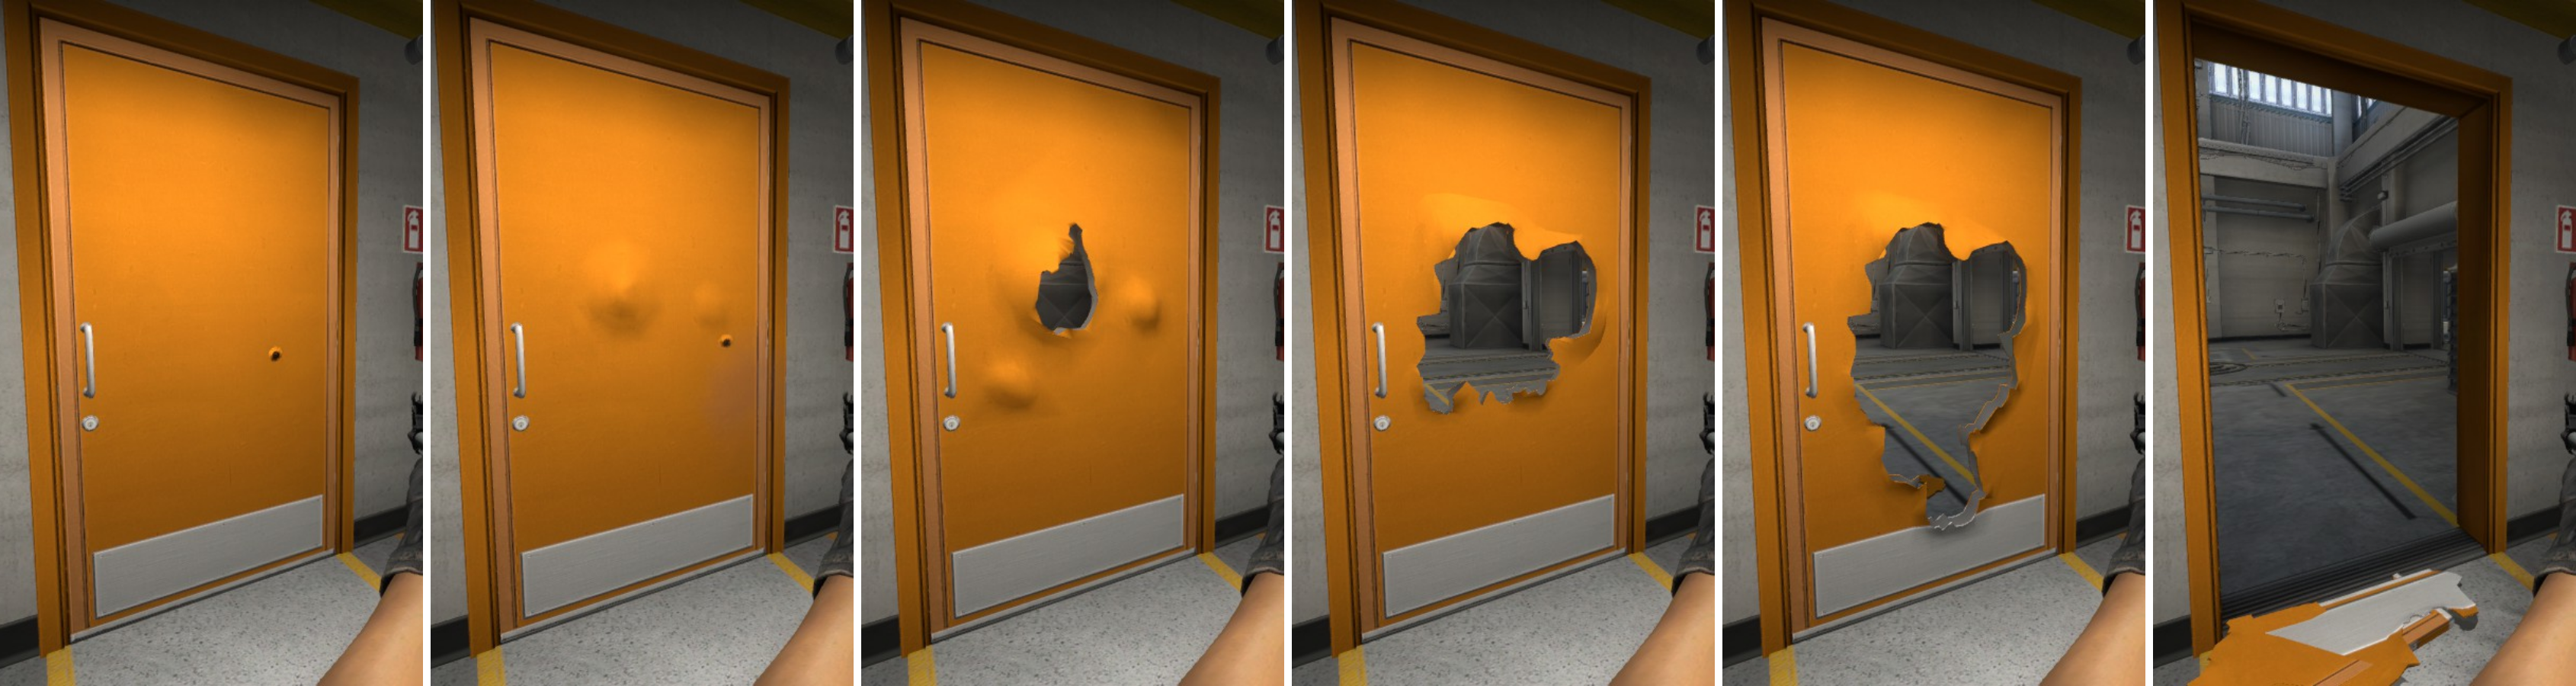
\includegraphics[width=\textwidth]{img/doors}
\caption{\emph{Source} engine swaps door models. Image taken from \emph{Counter Strike: Global Offensive}. Successively damaging any doors in the game will always produce this sequence of models, regardless of the exact point where the damage was applied.}
\label{fig:doors}
\end{figure}

\para{Height map approach} is closely intertwined with terrain generation. The basic principle behind modifying the environment with this method is changing the height of the terrain at given point. We can find this method used in the first 3D games that featured destructible terrain, \eg \emph{Magic Carpet (1994)}~\footnote{https://ultimatehistoryvideogames.jimdo.com/magic-carpet} or \emph{Starfighter 3000 (1994)}~\footnote{https://en.wikipedia.org/wiki/Star\_Fighter\_(video\_game)}.

The height map of a 3D terrain is represented as a uniform 2D grid \todo{of what values?}. The grind serves as a base \todo{kdyz reknes grid a base, tak se oponnt prepne do linearni algebry :D zjednodus to} of 3D space where each cell of the grid defines the terrain height in the respective column. A convenient approach is to use 2D grey-scale bitmap and represent the height as a colour distance from the white colour, black being the maximum. Because the grid only contains information about the discrete points, interpolation is used to create continuous terrain. We can also see \todo{view} this method as creating a function of two coordinates on the plane giving us the value on the vertical axis \todo{proc je potreba to viewovat jako funkci, pouzijes to pak nekde?}. The relative simplicity of the approach is counterweighted by the fact that it can only change the height of the terrain and does not allow creating caves, tunnels or similar hollow features.

\para{\emph{Geo-Mod}} (\emph{Geometry Modification Technology}\cite{geomod}) is an engine developed for the \emph{Red Faction (2001)}\footnote{http://redfaction.wikia.com/wiki/Red\_Faction} video game. It approaches the modification of the terrain by creating objects representing a void \todo{void tady znamena empty?} space. After every collision, a new object is created at the point of collision. This new object is then subtracted from the terrain creating the modified terrain with the newly created hole. The difference of the meshes is calculated in real time. Even though the engine does not work well with the buildings and other objects \todo{tusime proc?}, it represented the first significant attempt to create the fully destructible 3D environment that would work under real-time constraints.

\para{\emph{Geo-Mod 2}}~\cite{geomod}\footnote{Geo-Mod 2.0 presentation video https://www.youtube.com/watch?v=lICurOVsNv0} does not feature destructible terrain, instead, it focuses on realistic destruction of buildings. A set of smaller objects is used to represent each building as a ragdoll for the stress-based simulation model \todo{oponent v tomhle okamziku nevi co je ragdoll ani stress-based model}. Therefore every building needs to be specially prepared for this kind of physics simulation \todo{citation needed --- tady vubec neni jasny proc by to meli delat rucne; bylo by vhodnejsi popsat tvar vstupu toho algoritmu a cim se lisi od toho co by do ty hry slo jinak (predpokladam ragdoll (kterej grafici nezvladaj) vs. 3d model (kterej zvladaj ale nejde bourat)?)}. This process is done by hand in the development process and can not be modified at a runtime. The high complexity of simulation limits the engine in the scale of the game world and mutual proximity of destructible objects because \todo{v `because' neni moc zrejmy ze tam fakt je implikace, myslim ze spis tam chces `because of that, game avoids eg any interaction of multiple buildings'} it would require simulating the behaviour of multiple buildings at once.


\para{\emph{Frostbite}}~\footnote{http://www.frostbite.com/about/frostbite-3} engine (and mainly its component \emph{Destruction}~\cite{destruction}) is currently used in new mainstream games that feature destructible environment \eg \emph{Battlefield} series or \emph{Star Wars Battlefront (2015)}. It supports two different kinds of destruction micro-destruction on the surface and the large scale predetermined destruction on whole buildings. 

The dynamic micro-destruction focuses on creating small dents into the surface of the object. The dents are created dynamically at the point of impact and can be placed on any point of the surface.

For the large-scale destruction is focused \todo{english: For the....is focused?} on destroying entire buildings. The buildings are created from smaller parts that are linked together. Each part can disappear on its own (\cref{fig:frostbite}), and when there is not enough \todo{of what?} left, the whole building collapses. It does not use internal body stress or any physics \todo{`fyzika' ve hrach neni dobry podstatny jmeno, lepsi je It does not use any physical simulaiton ...} while doing this simulation. 

\begin{figure}
\centering
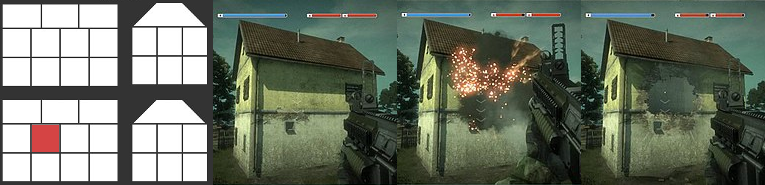
\includegraphics[width=\textwidth]{img/frostbite}
\caption{The arrangement of destructible elements for the large-scale destruction in \emph{Frostbite} engine (on the left). Rest of the images shows the process of large-scale destruction in \emph{Battlefield: Bad Company} implemented using \emph{Frostbite 1}.}\label{fig:frostbite}
\end{figure}

\todo{K obrazku s frostbite: Slo by na ty mapce vlevo oznacit ze si sejmul presne ten jeden ctverec?}

\section{Methods and algorithms}

Here we will give a short overview of several more rigorous algorithms commonly used for simulations of destructible environment. 

In simulations, we consider two types of objects: soft bodies and rigid bodies. A rigid body represents an object with a constant shape. It means \todo{`it means' neni uplne spravne davat do diplomky ani cesky jako `to znamena', zkus to v co nejvic pripadech nahradit tim ze ty vety slepis do jedny lepsi definice} that every two points on the body are always in the same relative position. On the other hand, soft bodies are deformable under an applied force, meaning a point on the body can change its position independently on every other point. Although there are no actual rigid objects in the real world, soft body simulation is computationally more expensive than the rigid body \todo{english: porovnavas simulaci s body}. Therefore, in the computer games, rigid body simulation is used almost exclusively. This brings us to the problem of imitating the soft body behaviour on a rigid body in the real-time simulation. \todo{brings us --- neslo by to rovnou pojmenovat tak ze soft body sice nedelame ale emulujeme je pomoci rigid bodies?}

It is worth mentioning that many soft bodies in the games players can not directly interact with, \eg waving flag or flowing water, are implemented as a pre-rendered animations and not actual simulations. The simulation of those objects would not bring any value from a gameplay perspective, but it would require a lot of processing power that could be used elsewhere. \todo{tohle je lepsi obratit: `kdyz uz setrime vykon, muzeme na soft bodies setrit i jinak, treba nektery nejsou worthy of interaction, tak se sice chovaj jako soft body ale sou fejkove predpocitany}

\subsection{Soft body deformation}
In this section, we will shortly introduce two different approaches for simulation of soft bodies. Despite the fact that soft bodies are currently not used in computer games to the extent of destructible environment \todo{to je docela silny tvrzeni, fakt neni zadna hra kde to neni?}, a few \todo{few/several/some?} soft body objects can show up in a game. We also expect that with an evolution of more powerful hardware, soft body deformation will make its way into the gaming world.
\label{sec:softBody}

\para{Finite Element Method} (FEM) is a numerical method used to simulate the behaviour of a system that can be modelled by solving the same \todo{which?} problem for the smaller discrete parts, called finite elements. Each element calculates its physical state, \eg stress or temperature, and propagates the results to neighbouring elements. This model can be used for simulation of fluid dynamics, brittle fractures~\cite{brittlefracture}, ductility~\cite{ductilefracture}, elasticity, heat transfer and other physical properties. It is beneficial in engineering, modelling and rendering scenes for computer generated images ~\cite{Bargteil:2007:AFE}. 
FEM requires a lot of computational resources and is mostly used in simulations that are not in real-time constraints. The algorithms like \citet{femingames} propose, that optimised version of FEM can be used in computer games. 

\para{Material point method} (MPM) is used to simulate the behaviour of continuum materials \todo{tohle je potreba prepsat aby z toho byla jasna definice continuum materialu}, continuum material is represented as continuous mass \todo{instead of? nebo aspon carku} not a set of discrete particles. MPM is a particle method \todo and uses material points (Lagrangian elements) to describe a body. Each material point stores and calculates its position, velocity and deformation gradient. The difference between MPM and FEM is that the MPM is a meshfree method. Meshfree method stores all its information in the particles and avoids numerical errors from remeshing algorithms. In the context of numerical method MPM is an Arbitrary Lagrangian–Eulerian numerical method \cite{ALE}, this means that calculations do not only use material points, but also a Eulerian grid. A simplified overview of algorithm steps follows, for more details see the thesis of \citet{jiang2015material}.
\todo{obecne tenhle celej odstavec je tak nejasnej ze aby clovek pochopil o co vlastne de tak musi preskocit na ten seznam, pak na obrazek, a kdyz selze i ten tak na ten clanek. Doporucuju prepsat, hlavne zduraznit cim presne se to odlisuje od FEM. Napr. tvrdis ze to nesimuluje set of discrete particles, a hned potom ze to je particle method?}

\begin{enumerate}
    \item Grid data are reinitialized to default values.
    \item Weights and weight gradients are computed on every particle.
    \item Mass and momentum are transferred from the particles to the grid.
    \item The explicit forces on nodes are calculated
    \item The explicit nodal velocity update is performed
    \item Grid based collision is performed on vertices.
    \item Particles are updated from grid velocities.
\end{enumerate}
These steps are illustrated in \cref{fig:mpm}.

MPM is useful for both fluid and soft body dynamics. It can simulate deformation, fractures, heat transfer, melting and other changes of the state of an object.

A popular example of MPM deployment can be seen in snow simulation in the \emph{Disney} film \emph{Frozen (2013)}. The simulation software \emph{Matterhorn}\footnote{https://www.disneyanimation.com/technology/innovations/matterhorn} computes the behaviour of different types of snow (\eg wet, fresh, sticky) and other materials, such as sand or mud.

\begin{figure}
\centering
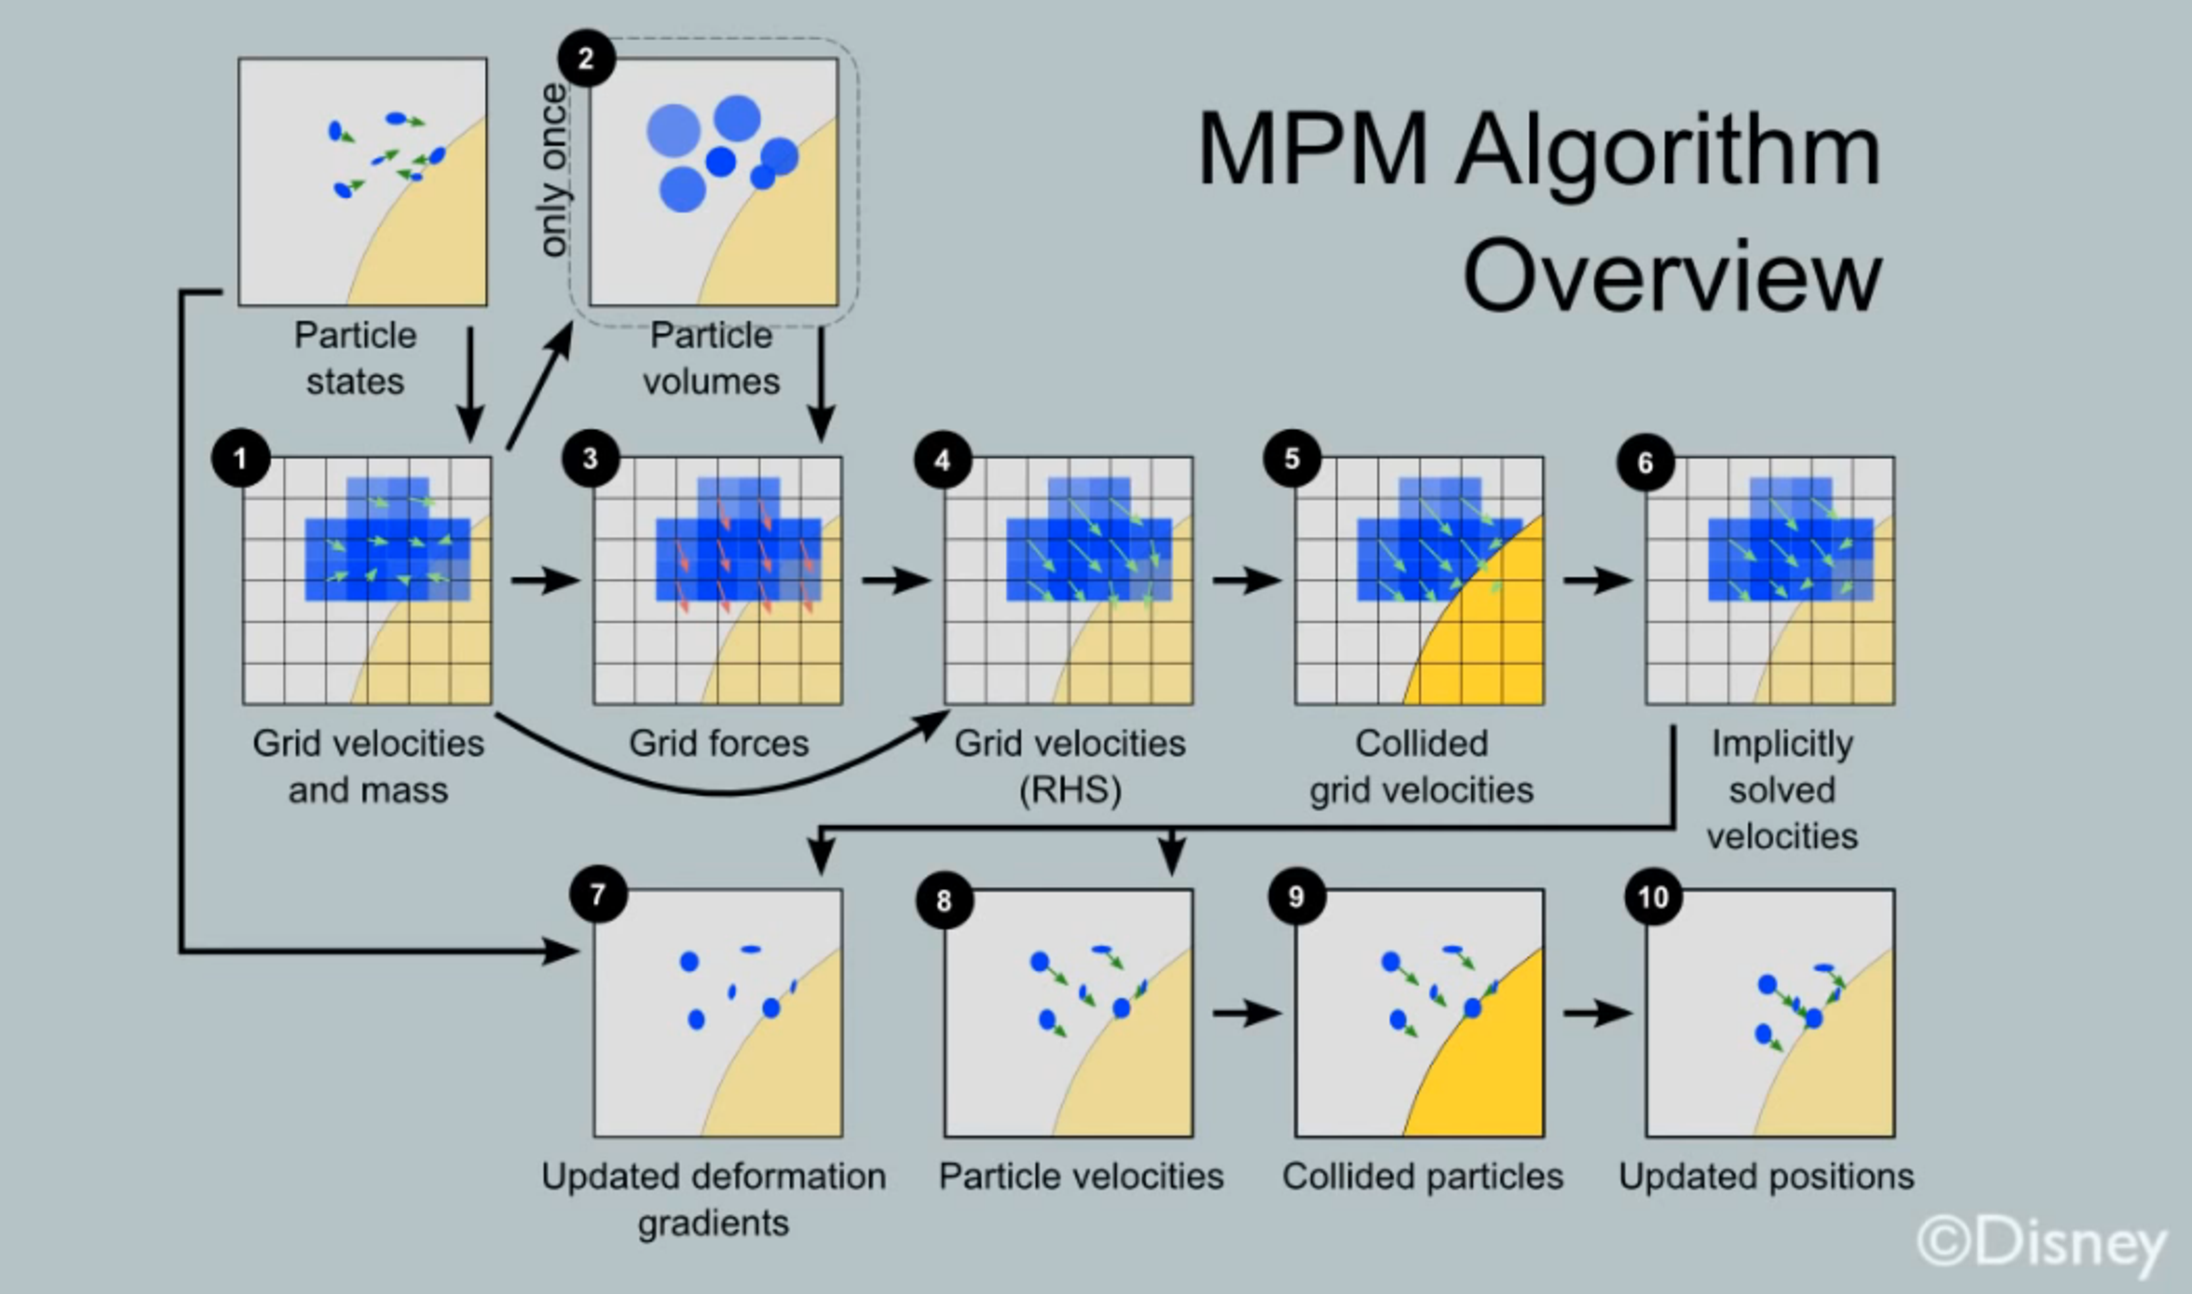
\includegraphics[width=\textwidth]{img/MPM}
\caption{Material point method algorithm overview. The top and the bottom rows operate in particle domain (Lagrangian) while the middle depicts grid-based (Eulerian) operations \cite{disney}.
}
\label{fig:mpm}
\end{figure}

\subsection{Rigid body decomposition}
In the soft body, application of the force propagates across the particles, and the connected particles break apart when the limit is exceeded. This creates the fracturing that may lead to the whole body splitting. In the rigid body simulation, the body has no internal structure, and therefore the applied force can only change the momentum of the entire body. This prohibits the deformation or fracturing a rigid body in a simulation.

To solve this problem, there are numerous approaches of decomposing the rigid body in the way that imitates fractures achieved by exceeding the elasticity of the soft material. The most common approach is a decomposition of a rigid body into smaller parts. A few \todo{some of. `A few of' znamena `aspon nejaky' ve smyslu `malo'. K jednotlivejm metodam to chce citace, a rovnou napis ze des mluvit jen o voronojovi pro demonstraci (pak muzes vynechat ten \\para u nasledujiciho odstavce, vypada stejne jako ty descriptiony coz je malinko matouci.} of the methods for decomposition are slicing by planes, convex decomposition, tetrahedralization and Voronoi tessellation.

\para{Voronoi tessellation} is a method of decomposing a solid object into smaller parts, as shown on \cref{fig:voro}. It is also applicable for \eg terrain generation~\cite{voronoiterrainrealtime}, but we will focus on object decomposition. Assuming the input is a closed triangular mesh with non-empty volume, the tessellation can be done in following three steps:

\begin{figure}
        \centering
        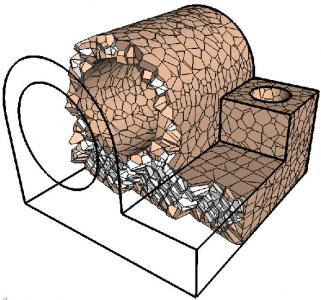
\includegraphics[width=0.4\textwidth]{img/clipped}
        \caption{The result of Voronoi tessellation \cite{yan2010efficient}}
        \label{fig:voro}
\end{figure}

\begin{description}
    \item[Delaunay tetrahedral decomposition] Given points $P$ in general position (the vertices of input mesh and a set of points inside its volume), tetrahedral mesh $DT(P)$ can be generated satisfying the following condition: no point in $P$ is inside the circumscribed sphere of any tetrahedra in $DT(P)$~\cite{cignoni1993parallel}.
    \item[Creating Voronoi diagram] For a Delaunay tetrahedral decomposition, its dual graph (with vertices in the centre of tetrahedrons circumscribed sphere) is a Voronoi diagram (see \cref{fig:voro}).
    
 \begin{figure}
    \centering
    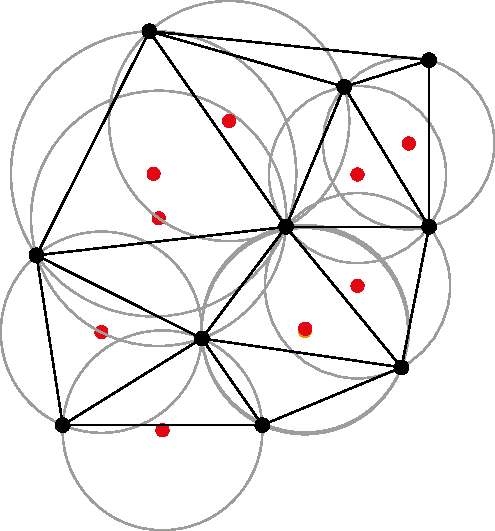
\includegraphics[width=0.4\textwidth]{img/delaunay}
    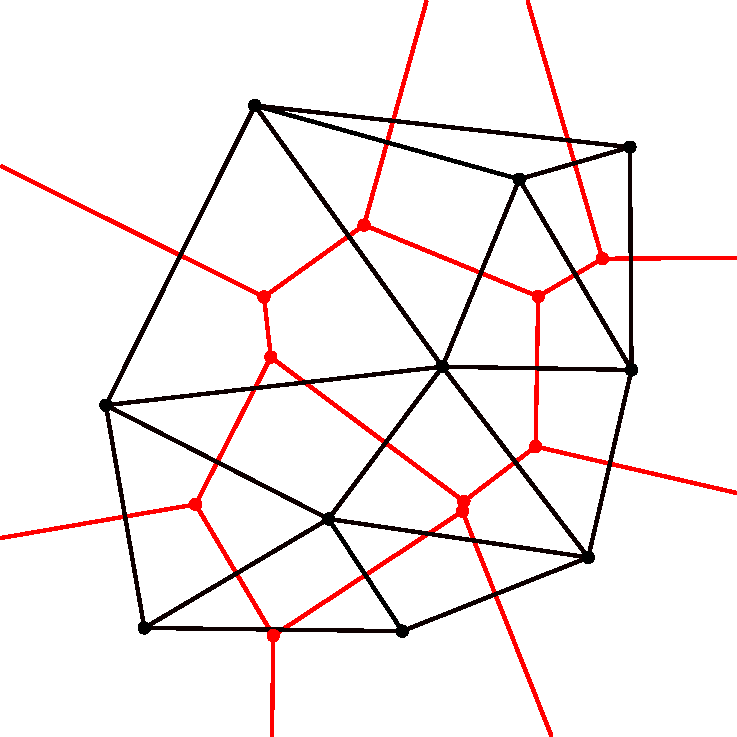
\includegraphics[width=0.4\textwidth]{img/voronoi}
    \caption{Transformation of 2D Delaunay triangulation to Voronoi diagram. Source: \url{https://en.wikipedia.org/wiki/Delaunay\_triangulation}}
    \label{fig:DT}
\end{figure}

    \item[Clipping the Voronoi diagram] Boundary cells of the Voronoi diagram are infinite (see \cref{fig:DT}) and need to be clipped by the original input triangular mesh. The efficient algorithm proposed by~\citet{yan2010efficient} for this task finds the intersection of the boundary Voronoi cell with the triangular mesh and continues with neighbourhood propagation to determine all intersections. 
\end{description}


\todo{co s tim? Jak je ten voronojuv tesselation rychlej, jaky sou vysledky? Nebylo by spatny dat \\ref na nejakou kapitolu kde to pouzijes.}

\section{Related research}
In this section we review two results of recent research that propose different techniques for environment destruction in computer games. First technique focuses on simulating the forces inside the object with the approach based on particle methods. The second one focuses solely on the destruction of rigid bodies with the use of Voronoi decomposition.

\subsection{A fast method for simulating destruction and the generated dust
and debris}
\label{sec:edem}
The method of \citet{edem} approaches destruction on three scales. At first, the destruction is performed on a coarse scale, and then the applied energy is used to calculate the amount and size of smaller debris and finally dust particles.

\begin{description}
\item[Destruction on a coarse scale] on this level the authors use Extended Distinct Element Method (EDEM) which is based on Element Method described in section \ref{sec:softBody}. Instead of using particles, EDEM uses a set of rigid bodies that need to be produced by some tessellation method. The extension over traditional DEM is the use of pore springs to connect the adjacent elements (see \cref{fig:spring}). The authors compare the elements to individual bricks (the distinct elements) held together by layers of mortar (the pore springs). If the applied force is sufficient to move the elements far enough from each other, the fracturing process is initiated. Pore springs also help the object retain its original shape after the force is applied. %after TIME. `applied force' neni time.
\begin{figure}[t] %h! a t dohromady si protirecej. Navic vsechny figuresy musej bejt refly z textu (jinak ctenar nevi kdy se na ne podivat a uplne je vynecha)
        \centering
        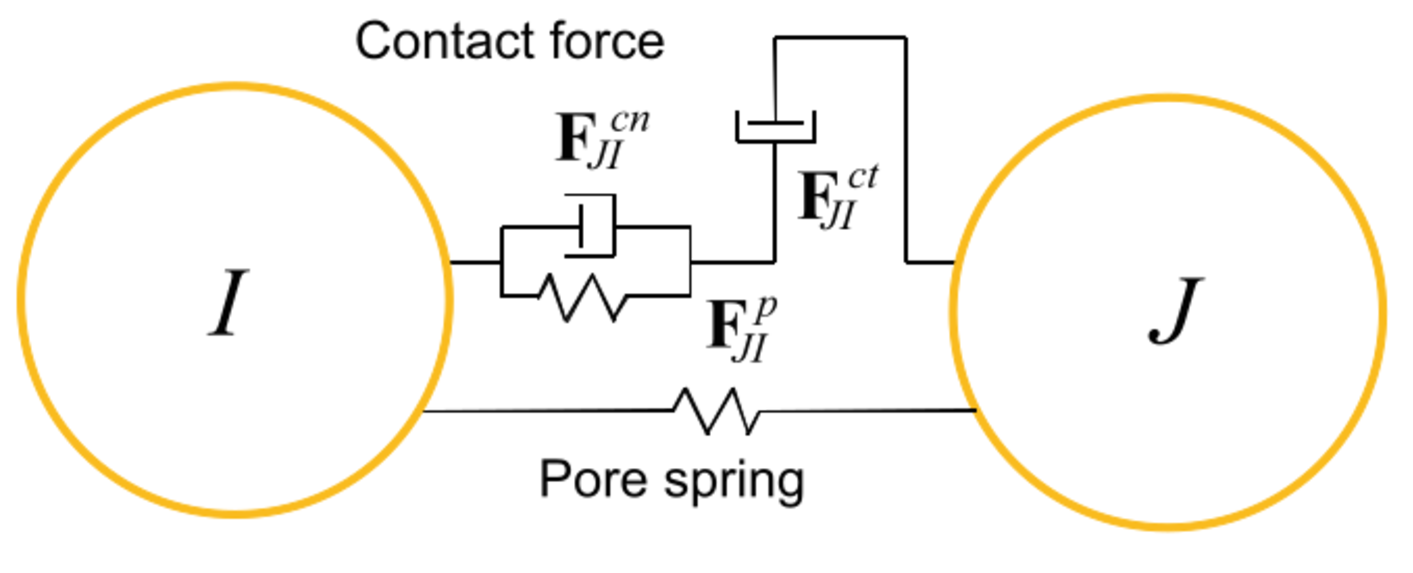
\includegraphics[width=0.7\textwidth]{img/spring}
        \caption{The force between two EDEM elements \cite{edem}}
        \label{fig:spring}
\end{figure}
\\Algorithm for creating EDEM elements
\begin{enumerate}
\item Represent the original object as a closed surface model.
\item Arbitrarily arrange the EDEM elements inside the object.
Elements are allowed to overlap at this point.
\item Move elements by performing the EDEM simulation. Only the contact force will be considered in this simulation.
\item Perform collision detection between the object’s surface
and elements, making sure that they always
stay inside the object.
\item Repeat (3)–(4) until elements are stabilised.
\item Construct a Delaunay diagram from the set of elements
and put the pore springs on the Delaunay edges that connect
the elements
\end{enumerate}
The position $\mathbf{x}_I$ and velocity $\mathbf{v}_I$ of the element $\mathit{I}$ can be found using Newton’s equation of motion as follows:
 
\[M\frac{d\mathbf{v}_I}{dt} = \sum_{J \in contact}^{} \mathbf{F}_{JI}^c + \sum_{K \in pore}^{} \mathbf{F}_{KI}^p + M\mathbf{g} \]
\[ \frac{d\mathbf{x}_I}{dt} = \mathbf{v}_I \]
Here, $\mathbf{g}$ is the gravitational vector, $\mathbf{F}^c_{JI}$ is the contact force, $\mathbf{F}^p_{KI}$ is the force due to the pore springs and $\mathit{M}$ is the element’s mass. Two elements \{I, J\} are in contact, if they are closer to each other than the diameter of a single element.

\item[Fine debris generation and simulation] If a fracture between EDEM elements happened, we can determine if there was enough energy to break EDEM element into smaller debris. The probability distribution is used to determine the size of debris. Debris is taken out of EDEM simulation and put into particle simulation, where each piece is represented as a particle without volume.

\item[Dust generation and simulation] Amount of generated dust is based on fracture energy and results of debris generation. Instead of simulating particles smaller than predetermined margin, they are represented as dust in a grid-based fluid simulation. The density of particular cell represents the amount of dust.

\end{description}
 \begin{figure}
        \centering
        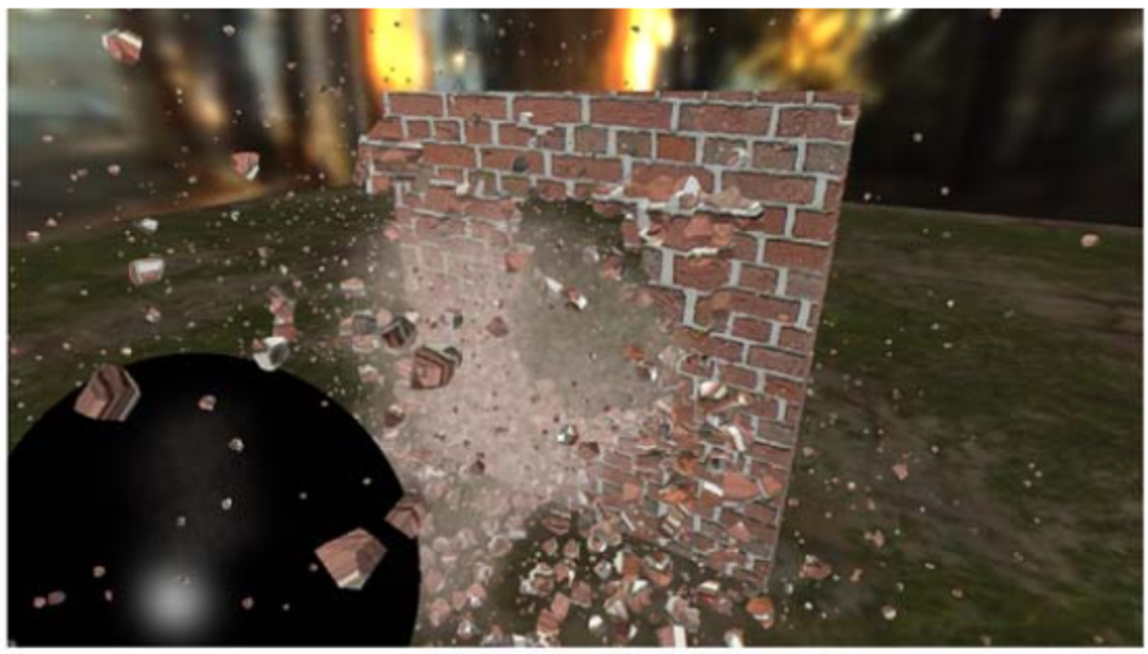
\includegraphics[width=0.49\textwidth]{img/edem_real}
        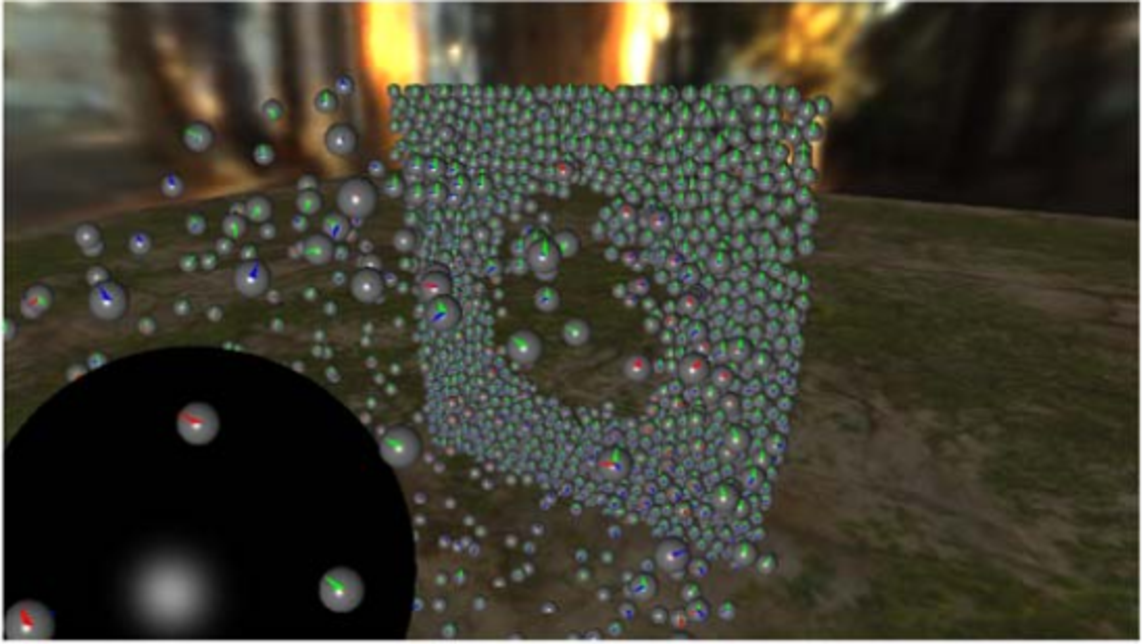
\includegraphics[width=0.49\textwidth]{img/edem}
        \caption{Result of this method with generated dust and debris (left) and EDEM elements (right) \cite{edem}}
        \label{fig:edem}
    \end{figure}
   
\begin{table}[ht!]
    \begin{center}
  \begin{tabular}{cc} 
  \parbox[b]{4em}{\centering EDEM\\elements} & FPS \\
  \hline
  128 & 320 \\
  256 & 160 \\
  512 & 75 \\
  1024 & 30 \\
  2048 & 9.1 
  \end{tabular}
  \end{center}
  \caption{Performance of EDEM element method without rendering \cite{edem}}
  \label{table1}
\end{table}
In conclusion, based on \cref{table1}, the frames per second (fps) drop proportionally with growing number of EDEM elements. The method achieved interactive fps on moderate number of EDEM elements. In addition, the proposed debris and dust generation can be combined with other methods.

\todo{Co se chce ukazat tim obrazkem 1.7? Bylo by dobry popsat ten rozdil na kterej ma clovek koukat, ktera metoda je vlevo a ktera vpravo (nebo to je ta sama metoda jen jinak zobrazena?). Btw s kterou casti textu souvisi? neni linknutej odnikud. Tabulky jsem predelal do svetove doporucenyho formatu tabulek.}

\subsection{Real Time Dynamic Fracture
with Volumetric Approximate Convex Decompositions}
\label{sec:RTDF}
The approach of \citet{nvidia} does not try to simulate the internal forces of an object and focuses only on rigid body decomposition. The idea behind this method is to represent the mesh as a compound shape of convex parts. The algorithm used for convex decomposition is Volumetric Approximate Convex Decomposition (VACD), which works by introducing the Voronoi decomposition into a bounding box of the mesh and then clipping the Voronoi cells by the mesh. The fracture pattern \todo{chybi definice fracture patternu} is precomputed and represented as a set of convex cells. The algorithm works as follows (the process is visualised in \cref{fig:vacdalg}:
\begin{enumerate}
\item The fracture pattern is aligned with the point of impact, and rotated and scaled randomly to avoid an occurrence of same-looking patterns.
\item The intersections of all cells with all convex parts are computed. To compute the intersection of a single cell with a single convex part, the convex part is clipped against all the planes of the cell one by one. 
At the end of this step, we have a set of new convex parts, and each convex part belongs to exactly one cell.
\item If there are convex parts that together entirely fill one cell, we can combine them into single new one convex part. The test is carried out using a simple volume comparison.
\item All convex parts that belong to one cell are combined to form a new compound part. This ensures that the temporary parts of decomposition into compound shape are not visible after the fracture (see \cref{fig:vacdfracture}).
\begin{figure}
        \centering
        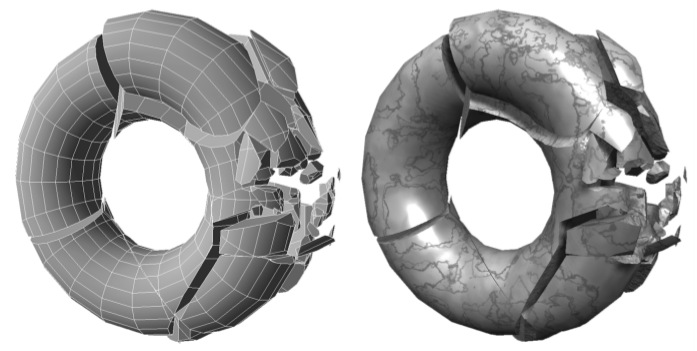
\includegraphics[width=0.7\textwidth]{img/vacdfracture}
        \caption{The decomposition to the
initial compound mesh does not become visible when a fracture
pattern is applied. Source: \citet{nvidia}}
        \label{fig:vacdfracture}
\end{figure}
\item Finally, the separate islands of convex parts are detected and individual compound shapes are constructed for them.
\end{enumerate}

\begin{figure}
\centering
        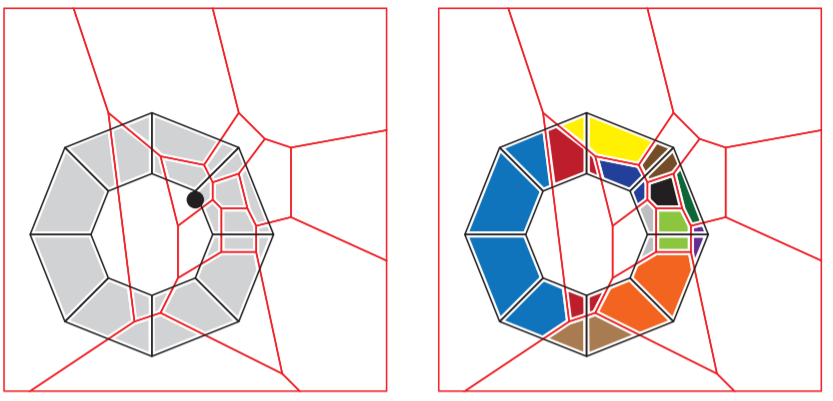
\includegraphics[width=\textwidth]{img/vacdAlgorithm}
        \caption{Overview of the fracture algorithm. Left: The fracture pattern (red) is aligned with the impact location (black dot). Middle: All
convex pieces are intersected with all cells. The green convex pieces can be welded to form a single piece because they cover the entire
cell. Pieces within one cell become a new compound (colouring). Island detection finds that the dark red compound needs to be split. Source: \citet{nvidia}}
        \label{fig:vacdalg}
\end{figure}

\todo{v tom obrazku: Become a new compound je to The compound, nebo Compound piece? (Taky neni jasny jak s tim souvisi coloring v zavorce)}

The cost of fracturing in this method depends only on the number of mesh triangles of the object being fractured and the resolution of fracture pattern. The paper suggests that the model with $10^6$ vertices and $5\cdot10^5$ faces can be fractured under 50ms. This makes this method suitable for real-time computer games.


\chapter{Related work}

\section{A fast method for simulating destruction and the generated dust
and debris}
This method \cite{edem} approaches destruction on three scales. At first, the destruction is performed on a coarse scale, and then the applied energy is used to calculate the amount and size of smaller debris and finally dust particles.

\begin{enumerate}
\item Destruction on coarse scale \\ on this level we use Extended Distinct Element Method (EDEM) which is based on Element Method described in the first chapter. The behaviour of the entire system is calculated based on interactions of individual elements. EDEM extends the method formerly using only contact force by adding pore springs connecting the adjacent elements. If we imagine the elements as individual bricks, then the pore springs represent a mortar holding them together. If the applied force is sufficient and elements move apart far enough, the fraction takes place. Pore springs also help the object retain its original shape after applied force.
\begin{figure}[ht!]
        \centering
        %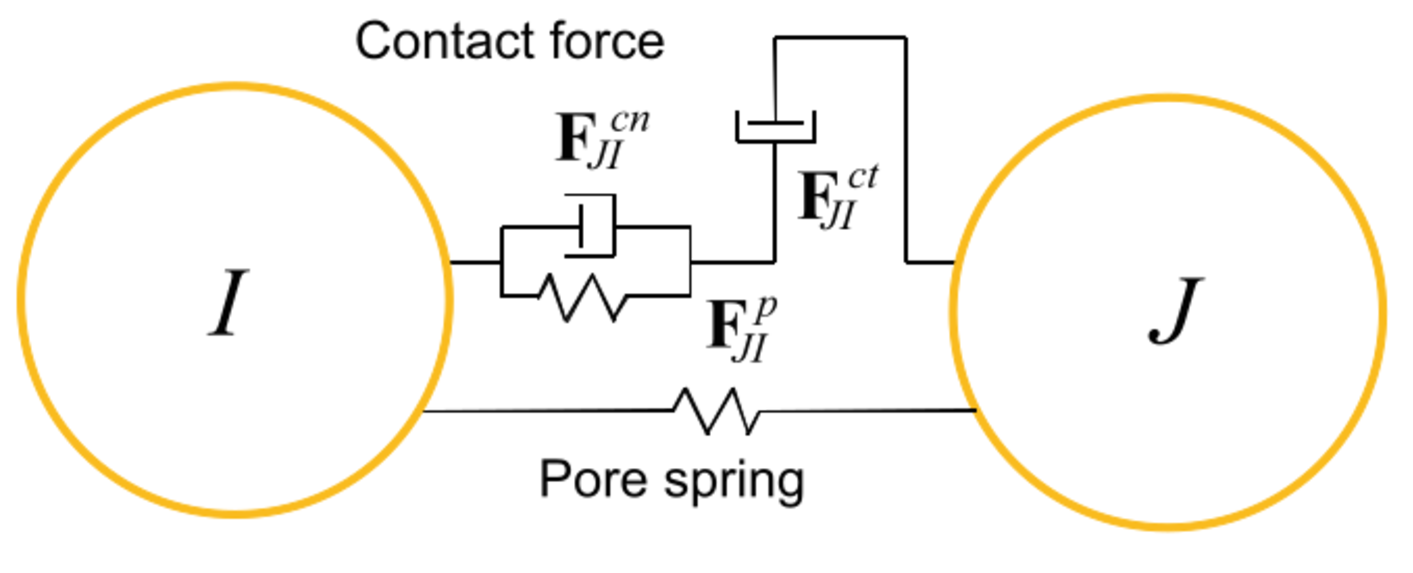
\includegraphics[width=0.7\textwidth]{img/spring}
        \caption{The force between two EDEM elements \cite{edem}}
        \label{spring}
\end{figure}
\\Algorithm for creating EDEM elements
\begin{enumerate}
\item Represent the original object as a closed surface model.
\item Arbitrarily arrange the EDEM elements inside the object.
The elements are allowed to overlap at this point.
\item Move the elements by performing the EDEM simulation. However, we only consider the contact force in this simulation.
\item Perform collision detection between the object’s surface
and the elements, making sure that the elements always
stay inside the object.
\item Repeat (3)–(4) until the elements are stabilised.
\item Construct a Delaunay diagram from the set of elements
and put the pore springs on the Delaunay edges that connect
the elements
\end{enumerate}
The position $\mathbf{x}_I$ and velocity $\mathbf{v}_I$ of the element $\mathit{I}$ can be found using Newton’s equation of motion as follows:
 
\[M\frac{d\mathbf{v}_I}{dt} = \sum_{J \in contact}^{} \mathbf{F}_{JI}^c + \sum_{K \in pore}^{} \mathbf{F}_{KI}^p + M\mathbf{g} \]
\[ \frac{d\mathbf{x}_I}{dt} = \mathbf{v}_I \]
Here, $\mathbf{g}$ is the gravitational vector, $\mathbf{F}^c_{JI}$ is the contact force, $\mathbf{F}^p_{KI}$ is the force due to the pore springs and $\mathit{M}$ is the element’s mass. Contact contains elements \{I, J\} if they are closer than the diameter of a single element, while pore
contains a pair of elements \{I, K\} when they are connected by a pore spring.

\item Fine debris generation and simulation \\after fracture between EDEM elements we can determine if the energy was big enough to break EDEM element into smaller debris. The Gaudin-Schuhmann distribution is used to determine the size of debris. Debris is taken out of EDEM simulation and put into particle simulation, where each piece is represented as a particle without volume.

\item Dust generation and simulation \\ amount of generated dust is based on fracture energy and results of debris generation. Instead of simulating particles smaller than predetermined margin, they are represented as dust in a grid-based fluid simulation. The density of particular cell represents the amount of dust.

\end{enumerate}

 \begin{figure}[ht!]
        \centering
        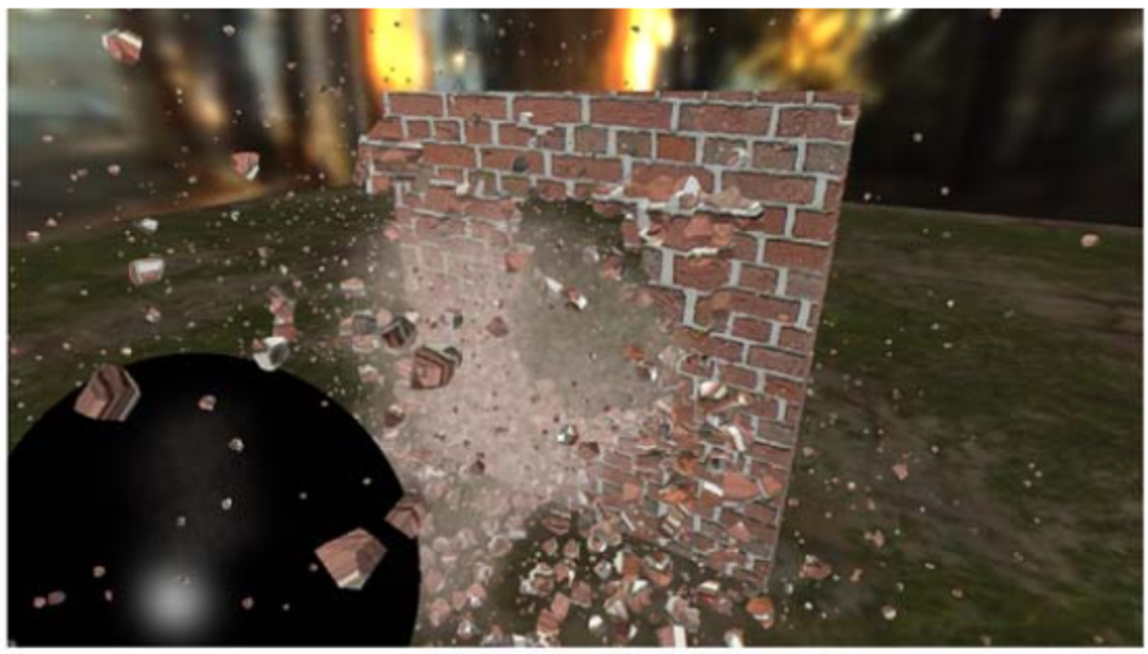
\includegraphics[width=0.49\textwidth]{img/edem_real}
        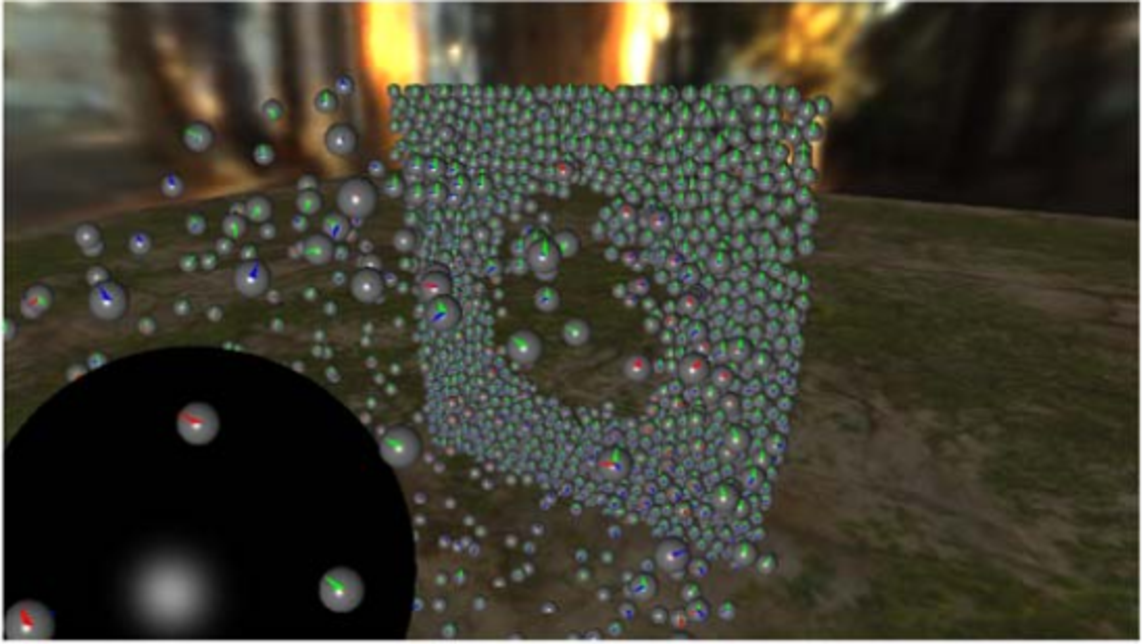
\includegraphics[width=0.49\textwidth]{img/edem}
        \caption{Result of this method with generated dust and debris (left) and EDEM elements (right) \cite{edem}}
        \label{edem}
    \end{figure}
   
\begin{table}[ht!]
    \begin{center}
  \begin{tabular}{ |l|c|c|c|c|c| } 
  \hline
  EDEM elements & 128 & 256 & 512 & 1024 & 2048 \\ 
  \hline
  FPS & 320 & 160 & 75 & 30 & 9.1 \\ 
  \hline
  
  \end{tabular}
  \end{center}
  \caption{Performance of EDEM element method without rendering \cite{edem}}
  \label{table1}
\end{table}
In conclusion, based on table \ref{table1}, the frames per second (fps) drop proportionally with growing number of EDEM elements. That makes this approach unusable in large scale environments in real time game which demands constant 30fps at least.

\section{Real Time Dynamic Fracture
with Volumetric Approximate Convex Decompositions}
\cite{nvidia}



















\chapter{Implementation Design}
\label{chaptImplementation}
In this chapter, we will introduce the implementation of our demo game and explain the basic principles and algorithms behind it. Then we will show a set of experiments testing the performance of the implementation and used algorithms.

After consideration of the various approaches implemented in games and also proposed efficient solutions to the problem of real-time destructible environment, we decided to implement and test a combination of reviewed techniques.  

At first, we considered implementation based on \emph{A fast method for simulating destruction and the generated dust and debris} (see \cref{sec:edem}). However, after degrading performance issues~\cref{sec:testing} we decided to abandon this approach.

Our approach is similar to \emph{Geomod} (described in \cref{sec:common}) and \emph{Real Time Dynamic Fracture with Volumetric Approximate Convex Decompositions}(RTDF) (described in \cref{sec:RTDF}), but with several key differences described below. 

\section{Main algorithm}
As mentioned, our algorithm will use boolean operations similarly to \emph{Geomod}, but applied to rigid body objects. The shape of removed object will be determined by Voronoi cell that will be generated dynamically for every collision. The collision information is received from the physics engine.

Our approach generates Voronoi cell at the point of collision. Then the difference of original mesh and the Voronoi cell is calculated and represents the damaged object. To generate the debris, the intersection of original mesh and the Voronoi cell is calculated. This action effectively cuts the object into two or more pieces, all of which are put back into simulation and can be damaged again (see \cref{fig:subtraction}). The Voronoi cell was chosen because it has easily randomizable shape and provides aesthetically good results. This choice is in no way critical to the rest of algorithm, and any other closed mesh can be used as well.

Similarly to the RTDF approach, the cost of fracturing in our implementation is solely dependent on the size and complexity of the fractured object~\cref{sec:testing}. This makes the method suitable for use in computer games with a large number of simple objects with low polygon meshes.

\begin{figure}
        \centering
        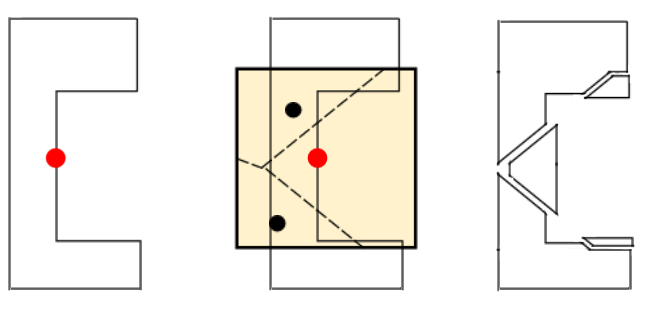
\includegraphics[width=\textwidth]{img/subtractionProcess}
        \caption{object with point of collision (left), generated Voronoi cells (centre), object divided into five new smaller objects after subtraction of the Voronoi cell belonging to the point of collision (right)}
        \label{fig:subtraction}
\end{figure}

To generate the Voronoi cell, we create a closed domain with the centre at the point of collision. In the domain, we need to create random points for generation of their Voronoi cells, and we also add the point of collision. Now we can use a Voronoi cell belonging to the point of collision as the object we subtract from the object in the collision. The boundaries of the domain clip the generated Voronoi cell, therefore the Voronoi cell can never be larger than the domain. Randomization of the size and shape of a Voronoi cell guarantees different result after every collision.

\section{Program Structure}
The main program loop runs in following steps:
\begin{enumerate}
\item Perform a step in physics simulation.
\item Handle collisions and perform destruction, see \cref{sec:collisions}.
\item Read user input and then apply correct forces to controlled vehicle.
\item Render current state of objects. In this step, a graphical representation of every object is updated to comply with its rigid body version.
\end{enumerate}

\begin{figure}
        \centering
        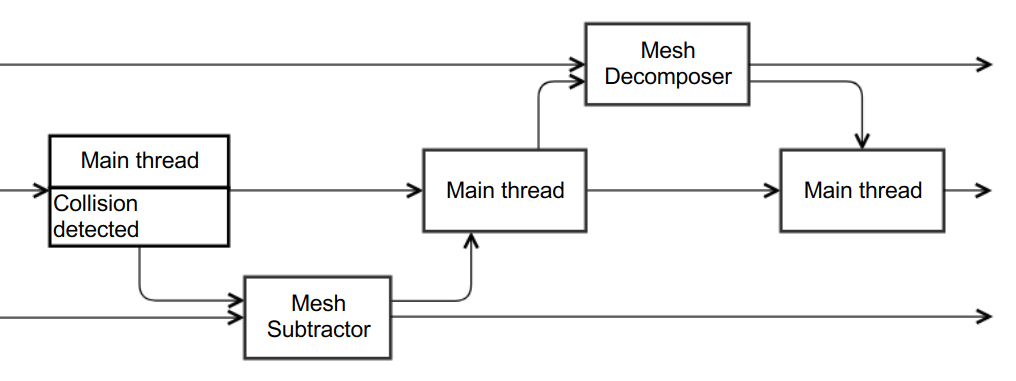
\includegraphics[width=\textwidth]{img/decompositionFlow}
        \caption{Diagram is showing multiple threads handling collision event. }
        \label{fig:threads}
\end{figure}
To make the simulation faster, we execute the most costly tasks asynchronously in separate threads. These tasks are convex decomposition and mesh subtraction. As a result, the program is running in three threads (\cref{fig:threads}): the main thread, a thread for subtracting meshes and a thread for decomposing triangular mesh into a set of convex shapes (\cref{sec:decomposition}). Both subtraction and decomposition threads communicate solely with the main thread, and all communication is done in producer-consumer model. Figure \ref{fig:objectInThreads} shows the changes of the object and its collision shape across all threads.

We use only one thread for all mesh subtraction tasks because we anticipate that the most of the consecutive collisions are going to be triggered by the same object --- shooting at one building multiple times in a row. In this situation, one subtraction does not have valid input data until the previous one has finished, which leads to sequential processing.

A use of a larger thread pool could be useful for convex decomposition. The conflicting state in a decomposition means that the object has changed since our calculation started and a new decomposition task was created. We do not know whether the newer task has already finished or not, but we know for certain, that if we discard our decomposition, the object has either temporary shape or a new valid decomposition. We did not implement a thread pool solution because we did not see it necessary and our hardware was not well suited for running more than four simultaneous threads.

\begin{figure}
        \centering
        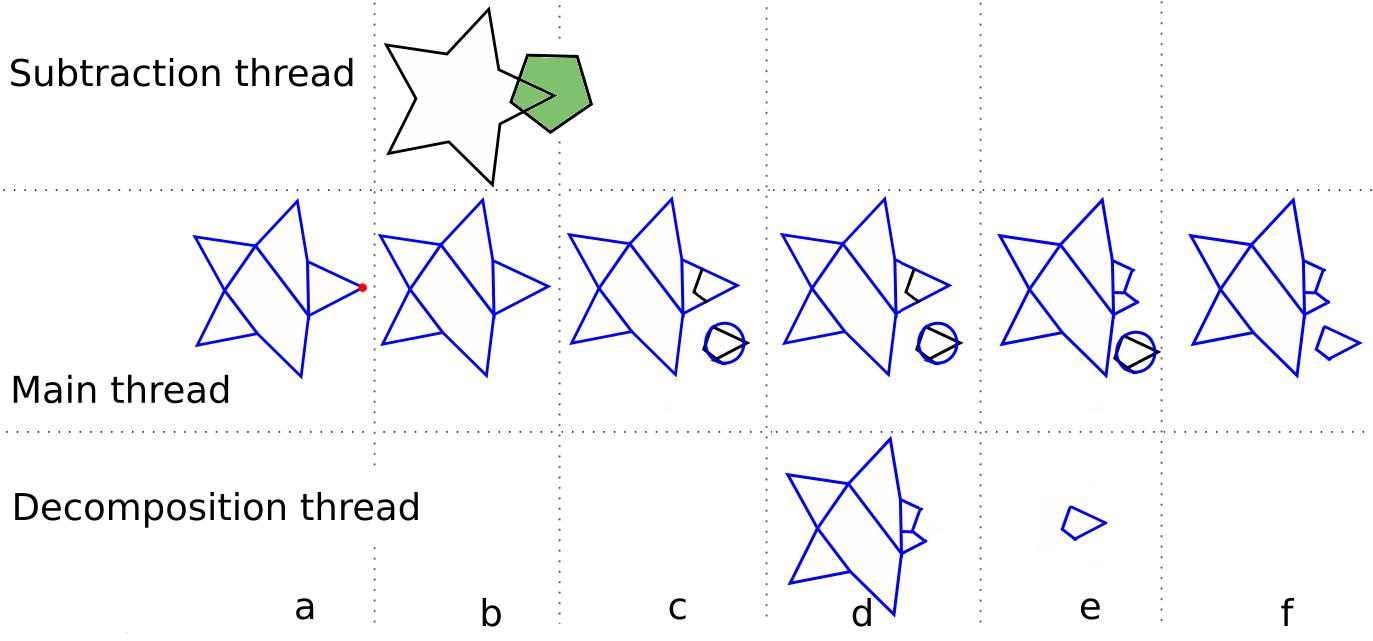
\includegraphics[width=\textwidth]{img/object-progress}
        \caption{Simplified overview of collision handling across multiple threads in simultaneous time slots. a) collision was detected (red), b) Voronoi cell (green) is being subtracted from the original mesh (black) in subtraction thread, c)the result of subtraction are two objects --- one one without change in collision shape (blue) and one with temporary spherical shape, d) and e) new collisions shapes are computed in decomposition thread, f) final result}
        \label{fig:objectInThreads}
\end{figure}

\section{Collision handling}
\label{sec:collisions}
After the collision, physics engine gives us a reference to two rigid bodies participating in the collision, point of collision and vector of force. For simplification, we will consider only one object, the point of impact and the force.

At first, we need to filter out unwanted collisions (collisions that should not damage the object). Those collisions can be results of an object placed on ground or collisions with not enough force to damage the object. 

For every collision we decide to perform destruction on, we generate Voronoi cell as described before, and move meshes of both objects into a task for mesh subtraction thread. After enqueuing all collisions, we can check if there are any prepared subtraction results for further use. The result of one subtraction task is a set of meshes that represent new objects. For every mesh, we create a new object, but we do not have its convex decomposition for the physics engine to perform accurate collision detection. Because the decomposition can take relatively long, we create a simple temporary collision shape (\eg sphere) for the new objects and keep using the current collision shape for the original object. Then we create tasks for decomposition of current meshes into new collision shapes and proceed with simulation, not waiting for the result. Decomposition is done in a separate thread, and the result is returned to the main thread where we check for decomposed shapes. With the shape ready in the main thread we replace the temporary shape for compound shape consisting of convex parts.

This process guarantees that we do not wait for either subtraction or decomposition and therefore we can have stable fps in our game.  It is better for the gameplay to have stable fps and lag behind with the simulation because poor performance in the main loop of the games makes the game stuttering. Meanwhile, a destruction happening a few frames later can be covered in animations of dust. To ensure consistent behaviour of new objects (we can put them into the simulation, and they do not fall through each other or otherwise not comply with laws of physics) when using a temporary collision shape, we need to make the temporary shape resemble the mesh as much as possible.  For the already existing objects keeping the older collision shape for a while longer should not disturb the simulation as the closest objects to this space are a newly generated object, those should be thrown away from the point of collision either way. For the new object, we use the sphere with the diameter equal to the shortest edge of the objects bounding box, meaning that the newly created objects have smaller collision shapes than meshes. The experiments showed that this factor does not visually impact simulation and the presence of the collision shape ensures that the object will not fall through other objects. 


\section{Convex Decomposition}
\label{sec:decomposition}
Regardless of used physics engine, our objects are represented as triangular meshes. Implementing mesh to mesh collisions is possible, but highly impractical. Even if checking every vertex of one mesh against all vertices of second mesh is sufficient, the complexity of algorithm would be dependent on the number of vertices. We can imagine a cube made out of eight vertices and the second cube with the same size but subdivided surface into thousands of vertices. Mesh to mesh collision detection algorithm would perform differently on the seamlessly identical objects. This behaviour is not desired in computer games where the surface of the objects is usually subdivided into thousands of triangles to created small details on a mesh.

To be able to perform fast mesh to mesh collisions we must find a way to describe the object as a set of geometrically simpler shapes. The convex shapes are the easiest for detecting mutual intersections, but encapsulating whole mesh into a convex hull would produce imprecise collisions. This problem is solved by performing a convex decomposition. Convex decomposition process splits the input object into a set of convex shapes, forming a compound shape. Now the complexity of the collision algorithm depends on the number of convex parts. 

While the exact convex decomposition can still produce a significant number of convex parts~\cite{convexDecomp}, in the setting of a computer game, the speed of calculation is much more relevant than the precision --- small differences between collision shapes and visual meshes are not considered to be a problem. To be able to perform collision detection at real-time, many approximate convex decomposition algorithms that sacrifice some precision to gain performance have been proposed. One of those algorithms is \emph{Hierarchical Approximate Convex Decomposition} algorithm (see \cref{sec:decompositionLib}) which we decided to use.

\section{Measurements and experiments}
\label{sec:testing}

\subsection{Performance test}
To estimate the performance of our application, we measure a time it takes to compute certain tasks. We measured the time required to process subtraction task and a time of convex decomposition, each measured in its separate thread. Then we measured the time from the creation of subtraction task for one object, to the time the new collision shapes is applied after convex decomposition is done on the same object.

We recorded 580 collisions in a game world with buildings with following amounts of triangles: 7x60, 1x142, 1x104. We shot the buildings at random locations.

\begin{table}
	\centering
  \begin{tabular}{lll}
  & Average & 0.18s \\
  Subtraction time: & Median & 0.14s \\
  & Variance & 0.02s \\
  \hline
  & Average & 0,13s \\
  Decomposition time: & Median & 0.11s \\
  & Variance & 0s \\
  \hline
  & Average & 0,39s \\
  Overall time:& Median & 0,3s \\
  & Variance & 0,06s \\
  \end{tabular}
  \caption{Statistics of the times recorded real time for given tasks. The overall time is measured from the time of creating subtraction task, to the time of having a new convex decomposition for the object in collision.}
  \label{tab:performace}
\end{table}

\begin{figure}
\centering
\begin{tikzpicture}
  \begin{axis}
    [
    boxplot/draw direction=x,
    ytick={1,2,3},
    yticklabels={Subtraction, Decomposition, Overall Time}
    ]
    \addplot+[
    boxplot prepared={
      median=0.14,
      upper quartile=0.24259,
      lower quartile=0.091783825,
      upper whisker=0.46,
      lower whisker=0.03
    },
    ] coordinates {};
    \addplot+[
    boxplot prepared={
      median=0.114929,
      upper quartile=0.1292675,
      lower quartile=0.1094205,
      upper whisker=0.16,
      lower whisker=0.10
    },
    ] coordinates {};
    \addplot+[
    boxplot prepared={
      median=0.303041,
      upper quartile=0.41976,
      lower quartile=0.2415265,
      upper whisker=0.7,
      lower whisker=0.05
    },
    ] coordinates {};
  \end{axis}
\end{tikzpicture}
\caption{Box plot showing the distribution of the times (horizontal axis) it takes to perform given tasks (vertical axis)}
\label{fig:boxtimes}
\end{figure}



Our expectation is that less than half a second delay between collision and a rendering of new objects would be acceptable for a game and thanks to the separate thread solution would not impact the frame rate. The experiment confirms that on given input we can successfully meet this expectation.

The problem seems to by a high variance in overall time. This can be explained by the tasks waiting in the queue for processing and shows that our solution is not well suited for a fast sequence of collisions. The problem here is that after every collision only one subtraction task is created, but the number of decompositions is nondeterministic and depends on the shape of the destructed object, the generated Voronoi cell and the position of the collision. We propose the use of a thread pool to resolve the convex decomposition problem.

\subsection{Dependency of our method on the number of triangles}
We designed an experiment to measure a relationship between a number of triangles and out two tasks, mesh subtraction and convex decomposition. In the experiment we created five cubes, all of the same size and positioned in the same place. Then we started our application five times, each time with different cube, and measured the times of mesh subtraction and convex decomposition. All the collisions are generated by letting the cube drop on the ground. The result of the experiment are as followed:
\begin{table}
\centering
\begin{tabular}{r|r|r}
number of triangles & subtraction time (s) & decomposition time (s) \\
\hline
12 & 0.037 & 0.118 \\
108 & 0.0678 & 0.135 \\
588 & 0.134 & 0.261 \\ 
2700 & 0.386 & 2.362 \\ 
10092 & 1.211 & 12.007 \\
\end{tabular}
\caption{}
\label{tab:subtraction-decomposition}
\end{table}

\todo{mne to nepride zrovna prehladne... tie data su prilis daleko od seba na takyto graf}
\begin{figure}
\centering
\resizebox{\textwidth}{!}{%
\begin{tikzpicture}
  \begin{axis}
    [
	boxplot/draw direction=y,
    xtick={1,2,3,4},
    xticklabels={12, 108, 588, 2700},
    ]
    \addplot+[
    boxplot prepared={
      median=0.03609005,
      upper quartile=0.039086475,
      lower quartile=0.0343537,
      upper whisker=0.05,
      lower whisker=0.03
    },
    ] coordinates {};
    
    \addplot+[
    boxplot prepared={
      median=0.06526395,
      upper quartile=0.070043275,
      lower quartile=0.064723875,
      upper whisker=0.070043275,
      lower whisker=0.06
    },
    ] coordinates {};
    \addplot+[
    boxplot prepared={
      median=0.1335775,
      upper quartile=0.1341765,
      lower quartile=0.13317175,
      upper whisker=0.14,
      lower whisker=0.13
    },
    ] coordinates {};
    
    \addplot+[
    boxplot prepared={
      median=0.384889,
      upper quartile=0.391104,
      lower quartile=0.38266425,
      upper whisker=0.4,
      lower whisker=0.38
    },
    ] coordinates {};
  \end{axis}
\end{tikzpicture}
}
\caption{Relation between number of triangles (horizontal axes) and time required for subtraction task (vertical axes).}
\label{fig:triangletimes}
\end{figure}


\todo{second plot}


The experiment showed us the limits of our approach. For the mesh subtraction, we can tolerate meshes with the size of about 600 triangles and still not cross half a second. On the other hand, convex decomposition times grow significantly faster, and the 600 triangle mesh takes a second to decompose.


\subsection{Testing the concept of EDEM}
To test EDEM (described in \cref{sec:edem}), we set up a cube divided into 439 tetrahedrons. After introducing constraints to hold the tetrahedrons together, we experienced a drop from 60fps (set as an upper limit) to 13fps. Having a large number of elements connected with springs in the simulation can also trigger an undesirable behaviour, such as contractions, retractions and self-induced explosions of the object. Performance issues and problems with keeping elements in a stable state concluded that the approach was not suitable for our implementation.





%\chapter{Documentation}

\section{Title of the first subchapter of the second chapter}

\section{Title of the second subchapter of the second chapter}


\chapter*{Conclusion}
\addcontentsline{toc}{chapter}{Conclusion}

This thesis has reviewed currently used techniques used to simulate destructible environments, implemented a simple game environment to test some of the approaches and designed and measured an approach based on a combination of the reviewed techniques. Thesis brings following results and conclusions:

\begin{itemize}
\item We have successfully presented an approach that combines boolean operations on 3D objects and Voronoi tessellation. The performance experiment~\cref{sec:overallperformance} has shown that the visual experience have not been impacted by presenting destruction multiple frames later as a result of multiple thread solution with a delayed application.

\item The experiments have concluded that used techniques are viable for low polygon meshes. For the boolean operations, we could tolerate meshes with the size of about 2000 triangles.The convex decomposition has reached the critical time at around 1000 triangles. The limits have been measured by the experiment designed in the~\cref{sec:triangleperformance}.

\item We have learned that mesh to mesh collisions
\end{itemize}


\subsection*{Future work}
The implementation showed several points that might be viable as starting points for future research and work.
\begin{itemize}
\item We have used CGAL library to perform boolean operations on 3D meshes, the approach it implements has performed consistently, however CGAL is a geometric library and it is designed to provide a rich interface with multiple views on data. For the purpose of destructible environment we propose an library for boolean operations on 3D triangular meshes optimized for use in real-time environments.
\item The implementation has shown the problem of determining a centre of gravity for arbitrary closed 3D triangular objects with homogeneous distribution of mass, after dynamically creating new meshes.
\item We have not incorporated texture generation into implementation, instead we relied on lightning to show the objects features. The generation of the textures for the fragments of original textured object would benefit this work.
\item Most of the modern game engines do not perform stability analyses on the damaged objects. We have envisioned a independent stability analyses running in a separate thread, testing recently damaged objects.
\todo{ja by som kolizie lietadla vobec neriesil, keby to bola normalna hra tak to napise game over a done.}
\end{itemize}



%%% Bibliography
%%% Bibliography (literature used as a source)
%%%
%%% We employ bibTeX to construct the bibliography. It processes
%%% citations in the text (e.g., the \cite{...} macro) and looks up
%%% relevant entries in the bibliography.bib file.
%%%
%%% The \bibliographystyle command selects, which style will be used
%%% for references from the text. The argument in curly brackets is
%%% the name of the corresponding style file (*.bst). Both styles
%%% mentioned in this template are included in LaTeX distributions.

\bibliographystyle{plainnat}    %% Author (year)
% \bibliographystyle{unsrt}     %% [number]

\renewcommand{\bibname}{Bibliography}

%%% Generate the bibliography. Beware that if you cited no works,
%%% the empty list will be omitted completely.

\bibliography{bibliography}

%%% If case you prefer to write the bibliography manually (without bibTeX),
%%% you can use the following. Please follow the ISO 690 standard and
%%% citation conventions of your field of research.

% \begin{thebibliography}{99}
%
% \bibitem{lamport94}
%   {\sc Lamport,} Leslie.
%   \emph{\LaTeX: A Document Preparation System}.
%   2nd edition.
%   Massachusetts: Addison Wesley, 1994.
%   ISBN 0-201-52983-1.
%
% \end{thebibliography}


\appendix
\chapter{Documentation}

\section{Title of the first subchapter of the second chapter}

\section{Title of the second subchapter of the second chapter}

\chapter{Implementation internals}
\addtocontents{toc}{\protect\setcounter{tocdepth}{0}}
\label{app:implementation}

This section provides insights on the code from a programmer's point of view. We will not focus on algorithms here, as we already did that in \cref{chaptImplementation}. The main focus here is on data representation and division of code into multiple modules.

\section{Design and libraries}
Logically, the program consists of four components, they are Physics, Graphics, Mesh Manipulation and they are linked together by Controllers, see~\cref{fig:architecture}. In the following list, we explain the purpose and summarise used technology in each of them.
\begin{description}
\item[Physics] provides us with the simulation of our objects and collision detection. We use \emph{Bullet physics} to implement this component. 
\item[Graphics] is used for rendering the current state of the physics world. This module provides the output of our application to the user by means of \emph{Irrlicht engine}.
\item[Controllers] ask the Physics to step the simulation and provided collision data and give the information about the current state of the world to the Graphics. The Controllers also read the user input which is done by parts of \emph{Irrlicht engine}. Mesh Manipulation component is called to create new objects and react to the collision provided by the Physics.
\item[Mesh Manipulation] provides tools for creating objects, creating a Voronoi cell (done by \emph{Voro++}, converting data and handling the collisions. To be able to do the mentioned tasks, Mesh Manipulation works closely with \emph{CGAL} library and also use \emph{HACD} library for convex decomposition.
\end{description}

\begin{figure}
        \centering
        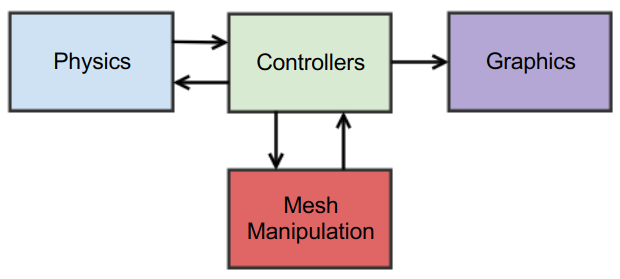
\includegraphics[width=0.7\textwidth]{img/architecture}
        \caption{Diagram showing architecture of the application}
        \label{fig:architecture}
\end{figure}

\section{Data representation}
As a result of using multiple libraries for a multitude of tasks, we have to deal with a lot of different data representations of the same objects. 

We will introduce the data structures that are used to represent one in-game object for multiple purposes. We can see how different data types are converted in~\cref{fig:conversions}.

\begin{figure}
        \centering
        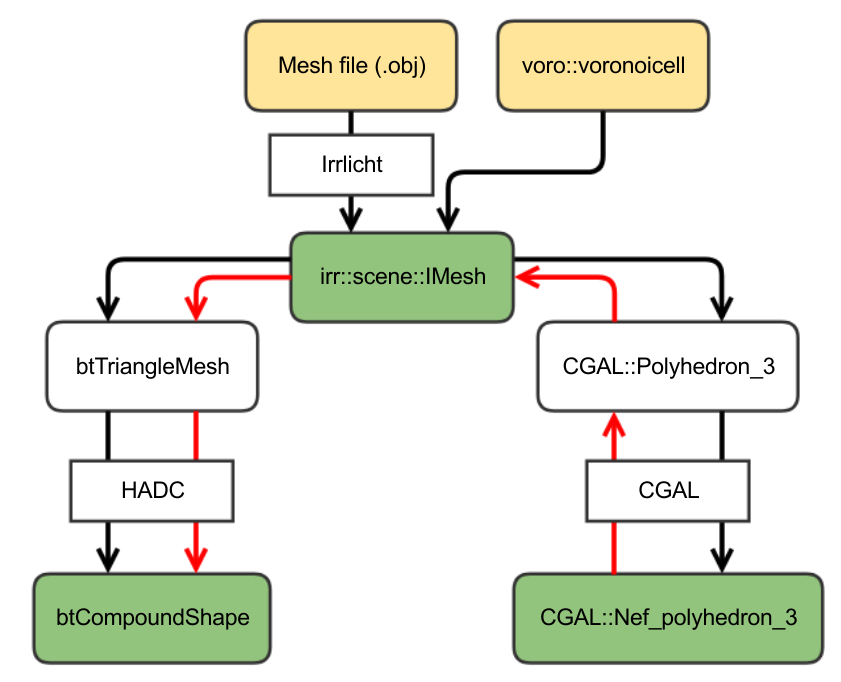
\includegraphics[width=\textwidth]{img/conversions}
        \caption{Data conversion diagram. Input formats - yellow, required formats - green. Black lines show used conversions, red lines show required process after a change of the shape of an object. Rectangles signify the library used to make the conversion, if none a member function of {\tt gg::MMeshManipulators} is used.}
        \label{fig:conversions}
\end{figure}

\subsection*{\tt btRigidBody}
\emph{Bullet physics} uses this class to hold information about a rigid collision object. For us, most important part of the body is a collision shape.

The collision shape can be of multiple types, most notably a convex hull or a primitive geometric shape, a triangular mesh or a compound shape. We need the collision shape to be as close to a visual mesh as possible. Because calculating collision between triangular meshes is not implemented in the \emph{Bullet physics} and would be too costly even if implemented, we choose the representation by compound shape.

One more parameter of {\tt btRigidBody} to consider is the object mass. Bodies with mass set to zero (or negative value) are considered static objects and do not move. Bodies with positive mass react to gravity and other external forces, their centre of gravity is set to their respective origin of local coordinates. This poses a problem when the origin is not inside the object. Our solution is to manually translate the mesh to the origin. \todo{ref link do kodu kde to delas}

\subsection*{\tt irr::scene::ISceneNode} 
Graphical object in the \emph{Irrlicht engine} is represented by this class. It is an abstract class instantiated into multiple types of graphical objects, \eg lights, cameras, animations, particle systems. We are using {\tt irr::scene::IMeshSceneNode} for our objects. The mesh information in {\tt irr::scene::IMeshSceneNode} is stored in {\tt irr::scene::IMesh}. 

\subsection*{\tt irr::scene::IMesh} 
This class stores the mesh information in multiple mesh buffers. Each buffer has an array of vertices and an array of indices. Every index in the array of indices refers to one vertex. However, we found out that not every vertex is referred to, and therefore valid. Indices divided into consecutive non-intersecting triples form a triangular face of a mesh. 

\subsection*{\tt CGAL::Nef\_polyhedron\_3}
\label{sec:nef}
"A Nef-poly-he-dron in dimension $d$ is a point set $P \subseteq \mathbb{R}^d$ generated from a finite number of open halfspaces by set complement and set intersection operations."~\footnote{http://doc.cgal.org/latest/Nef\_3/index.html\#Nef\_3Definition} In other words, {\tt CGAL::Nef\_polyhedron\_3} is a boundary represented data structure closed under Boolean operations. This make it ideal to perform our boolean operation on.
This structure imposes a restriction on the data we can use to represent our objects, the underlying halfedge data structure~\footnote{http://doc.cgal.org/latest/HalfedgeDS/index.html\#Chapter\_Halfedge\_Data\_Structures} is restricted to orientable 2-manifolds. A common examples of non-manifold geometry are: open geometry, two neighbouring faces with opposite normals, two faces sharing vertex but no edge, self intersecting geometry, inside faces.

\subsection*{\tt gg::MObject} 
{\tt gg::MObject} is a class designed to unite all data about one in-game object into one structure. It includes {\tt irr::scene::ISceneNode}, {\tt CGAL::Nef\_polyhedron\_3} and {\tt btRigidBody}. It implements the mechanism ensuring that upon deletion of an object, its parts are first removed from their respective engines, and then safely deallocated before {\tt gg::MObject} itself is destroyed.


\section{Modules}
In this section, we describe the functionality of each program module. Third party software is not be described here, details about used libraries can be found in \cref{chapt:technology}. Interactions between modules are visualised in \cref{fig:modules}. \emph{Irrlicht Engine} is not present in the diagram because we do not structurally depend on it. Every module is contained in a file of the same name, as a class with that name prefixed with letter M (\ie Object Creator can be found in file ObjectCreator.cpp and is implemented as class {\tt gg::MObjectCreator}). Also, namespace {\tt gg} identifies exact components of the application implemented for this thesis.

\begin{figure}
        \centering
        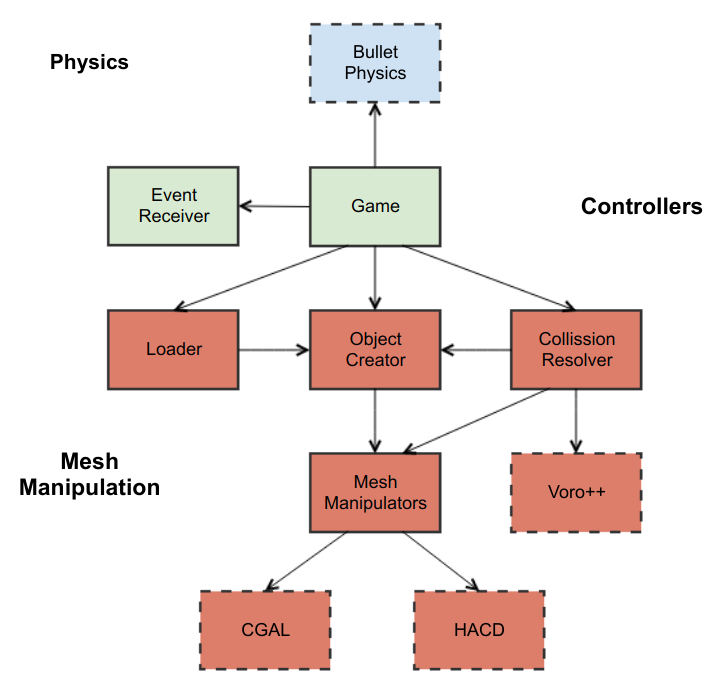
\includegraphics[width=\textwidth]{img/objectmodel}
        \caption{Software architecture shown on diagram of relationships of program modules. Third party software is highlighted in dashed rectangles.}
        \label{fig:modules}
\end{figure}

\begin{description}

\item[Game] module holds {\tt gg::MGame} class which is the core of the application. The communication with the physics engine,  the graphical engine and mesh manipulation parts of the software is managed from here.

\item[Event Receiver] module implements the instance of {\tt irr::IEventReceiver} from Irrlicht engine and it is used to read the user input.

\item[Loader] is only used for initializing the application. It parses the data that describe the game environment from the \emph{medial/world.cfg} file, constructs the objects using {\tt gg::MObjectCreator}, and returns the set of constructed objects.

\item[Object Creator] uses Builder pattern in order to initialize the data contained inside {\tt gg::MObject}, namely {\tt btRigidBody, CGAL::Nef\_polyhedron\_3} and {\tt irr::scene::ISceneNode}.

There are three member functions that allow us to create {\tt gg::MObject}s  with different behaviours from the same set of input parameters (see \cref{sec:data}). We can create a destructible object, an indestructible object with box collision shape and a rectangular indestructible object without input mesh.  Those functions are meant to be used exclusively for application initialization, as they generate a new {\tt CGAL::Nef\_polyhedron\_3} and convex decomposition from their mesh.

Two more kinds of objects can be created: a projectile that is shot from the given position with the given impulse and a destructible object with temporary collision shape (sphere shaped). Because the object with temporary collision shape is constructed while the game is being played and construction of {\tt CGAL::Nef\_polyhedron\_3} can take a longer time, we will construct it beforehand and then provide it to the Object Creator.

\item[Collision Resolver] implements the Collision handling process, described in~\cref{sec:collisions}. Conversions between data formats that are required during the process are externalised to Mesh Manipulators module to maintain the code readable.

\item[Mesh Manipulators] provides set of utility functions. Because different libraries are used for physics simulation, rendering and geometric manipulation, those functions provide means for converting data between different formats.
\end{description}


\chapter{Installation guide}
%\addcontentsline{toc}{chapter}{Appendix - Installation guide}
\addtocontents{toc}{\protect\setcounter{tocdepth}{0}}

This section is a manual to install the dependencies of our application. It is also a guide to compiling our source code. The whole section will focus on the installation process on \emph{Ubuntu 17.04}. The application is in no way limited to this single operating system and its version. Our code is written in \emph{}{C++14} standard and platform independent. All used packages are available for multiple \emph{Linux} distributions \eg \emph{Debian, Fedora, Gentoo }  and they are also open-source and can be manually compiled and installed on most of the operating systems.

\section{Installing packages}
We provide versions of packages used to create and test our implementation. It is not guaranteed whether newer or older versions of packages are compatible.
\begin{center}
\begin{tabular}{ |l|l| }
\hline
package & version \\
\hline
libbullet-dev & 2.83.7+dfsg-5 \\
libirrlicht-dev & 1.8.4+dfsg1-1 \\
libcgal-dev & 4.9-1build2 \\
voro++-dev & 0.4.6+dfsg1-2 \\
HACD & preferably use a copy distributed with our application\\
&downloaded from: https://sourceforge.net/projects/hacd\\
\hline
\end{tabular}
\end{center}

\section{Compiling and running the application}
Now we will provide the instructions to install our application. Fist we cover a simple installation using our prepared {\tt Makefile}s and then detailed instructions for manual compilation.

We assume that all the right versions of the packages from the previous section are correctly installed. The HADC library is included with our code with its {\tt Makefile}.

\subsection*{Using make}
First,  the HACD library needs to be compiled and then our application. The application consists of seven modules and can take a few minutes to compile. Consider using make -j$[N]$ to run parallel jobs.
\begin{code}
\~/bachelor_thesis\$ make -C lib/hacd/
\~/bachelor_thesis\$ make
\~/bachelor_thesis\$ build/game
\end{code}

\subsection*{Manual compilation}
Here we are going to exclusively focus on compiling our own code using a \emph{g++} compiler version 5 or higher, supporting {\tt c++14}. All of our {\tt cpp} and their respective header files can be found in {\tt /src} directory.
Following flags are needed to compile individual modules into object files:
\begin{code}
-std=c++14
-frounding-math
-isystem /usr/include/bullet 
-isystem /usr/include/irrlicht 
-isystem /usr/include/bullet/LinearMath 
-isystem include (HACD header files)
\end{code}

Linking object files to make a final application requires adding the following libraries: (HADC library also need to be linked to our application, link it as a static or dynamic library depending on installation.)
\begin{code}
-lIrrlicht 
-lBulletSoftBody 
-lBulletDynamics 
-lBulletCollision    
-lLinearMath 
-lvoro++ 
-lgmp 
-lCGAL 
-lCGAL_Core 
-lmpfr 
-lpthread
HACD.a or -lHACD (second option may require -L/path/to/library)
\end{code}
















%%% Figures used in the thesis (consider if this is needed)
%\listoffigures
% list of figures je dobrej do knizek co maj 500+ stranek, tady to je uplna zbytecnost.

%%% Tables used in the thesis (consider if this is needed)
%%% In mathematical theses, it could be better to move the list of tables to the beginning of the thesis.
%%%\listoftables

%%% Abbreviations used in the thesis, if any, including their explanation
%%% In mathematical theses, it could be better to move the list of abbreviations to the beginning of the thesis.
%%%\chapwithtoc{List of Abbreviations}

%%% Attachments to the bachelor thesis, if any. Each attachment must be
%%% referred to at least once from the text of the thesis. Attachments
%%% are numbered.
%%%
%%% The printed version should preferably contain attachments, which can be
%%% read (additional tables and charts, supplementary text, examples of
%%% program output, etc.). The electronic version is more suited for attachments
%%% which will likely be used in an electronic form rather than read (program
%%% source code, data files, interactive charts, etc.). Electronic attachments
%%% should be uploaded to SIS and optionally also included in the thesis on a~CD/DVD.
%%% Allowed file formats are specified in provision of the rector no. 23/2016.
%\chapwithtoc{Attachments}

\openright
\end{document}
